% ========================================= TEMPLATE INFO ========================================
%
% Author:       P4ntomime
% Version:      1.0.0
% Last updated: 2024-02-18
% Brief:        A LaTeX template for summaries. See README.md for more information.
% 
% ================================================================================================
\documentclass[8pt, a4paper, twoside]{extarticle}
% Font size:    8pt
% Paper size:   A4
% style:        twoside (needed, so odd and even pages have different margins)
% orientation:  portrait. (use 'landscape' for landscape orientation)


% ========================================= DOCUMENT INFO =========================================
\def\title{Regelungstechnik 1}           					% title
\def\shorttitle{RegT1} 										% short title (displayed as PDF title)
\def\dozent{Prof. Dr. Lukas Ortmann}         				% lecturer
\def\semester{HS 2026}     									% semester
\def\author{Simone Stitz, Mirko Ratti}        				% author(s)
\def\repo{https://gitlab.com/sstitz/regelungstechnik-1e}    % repository link
\def\version{3.0.\today}    								% version
\def\pagelimit{20}           								% page limit -> causes pages after limit to be red
\def\titleoption{normal}   									% options: compact, normal
\def\enableToC{true}

% ================================= PACKAGES, SETUP AND COMMANDS ==================================
% =========================================== PACKAGES ============================================
\usepackage[utf8]{inputenc}         % input encoding: UTF-8
\usepackage[T1]{fontenc}            % font encoding: T1
\usepackage{textcomp}               % additional symbols
\usepackage{times}                  % times new roman font
\usepackage[main=ngerman]{babel}    % set main language to german


\usepackage{multicol}               % provides multicols environment
\usepackage{geometry}               % set page layout


\usepackage{enumitem}               % list customization
\usepackage{outlines}               % easy nested lists
\usepackage{tabularx}               % some nicer tables with X columns
\usepackage{hhline}                 % double lines in tables
\usepackage{booktabs}               % thick and thin lines in tables


\usepackage{amsmath}                % math symbols
\usepackage{amssymb}                % more math symbols
\usepackage{mathtools}              % more math tools needed for pmatrix modification
\usepackage{mhsetup}                % needed to modify pmatrix environment
\usepackage{txfonts}                % Times math font
\usepackage[squaren]{SIunits}       % SI-units
\usepackage{bm}                     % bold math symbols
\usepackage{trfsigns}               % needed for "Laplace" symbol (Korrespondenz)
\usepackage{mathrsfs}               % needed for Fourier transform "F"
\usepackage{romannum}               % needed for roman numbers


\usepackage{graphicx}               % include graphics
\usepackage{graphbox}               % needed for aligning images in multicol environment
\usepackage{scalerel}               % scale any objects
\usepackage{anyfontsize}            % set any font size
\usepackage{xcolor}                 % needed for colors


\usepackage{tcolorbox}              % colored boxes
\usepackage[outline]{contour}       % contour for text (used in custom underline command)
\usepackage[normalem]{ulem}         % custom underline (used in custom underline command)


\usepackage{tikz}                   % needed for TikZ drawings


\usepackage{listings}               % for nicer code display
% to use nodes inside listing see: https://texample.net/tikz/examples/tikz-listings/


\usepackage{hyperref}               % clickable links
\usepackage{qrcode}                 % QR code generation (also clickable)


\usepackage{ifthen}                 % if-then-else commands
\usepackage{calc}                   % simple arithmetic in LaTeX commands


\usepackage{draftwatermark}         % watermark on pages after a certain limit
\usepackage{fancyhdr}               % custom header and footer
\usepackage[explicit]{titlesec}     % custom section titles


\usepackage{datetime2}              % custom date format for versioning


% ========================================== BASIC SETUP ==========================================

% --------------------------------------- DOCUMENT SETTINGS ---------------------------------------
\hypersetup{hidelinks,
% set pdf metadata
            pdfauthor={\author},
            pdftitle={\shorttitle},
            pdfsubject={\title\ \semester},
            pdfkeywords={Gahn go lerne!!}}

% set style for URLs
\urlstyle{same} % sets url font to the same as the preceeding text

% set page layout
\geometry{left=3mm, 
          right=3mm, 
          top=3mm, 
          bottom=6mm, 
          headheight=0mm, 
          headsep=0mm, 
          footskip=4mm}

\setlength{\columnsep}{1.5mm}       % distance between columns
\setlength{\columnseprule}{0.1pt}   % thickness of column separation line
\setlength{\parindent}{0pt}         % no paragraph indentation

\setcounter{tocdepth}{2}            % only display sections and subsections in toc
% \setcounter{secnumdepth}{0}       % uncomment to disable section numbering

\DeclareMathSizes{8}{8}{6}{5}       % set math font sizes for 8pt document


% --------------------------------------- COLOR DEFINITIONS ---------------------------------------
\definecolor{sectioncolor}{HTML}{f35832}
\definecolor{subsectioncolor}{HTML}{fabcad}
\definecolor{sectextcol}{HTML}{f5f5f5}
\definecolor{subsectextcol}{HTML}{000000}

\definecolor{backcolour}{HTML}{f5f5f0} % background color for highlighted text

% TODO: define color palette
% color palette: https://colorkit.co/color-palette-generator/FF8552-9e22bd-404E7C-C32E15-225A28/
\definecolor{green}{HTML}{1af430}
\definecolor{red}{HTML}{f90d09}
\definecolor{blue}{HTML}{093ce5}
\definecolor{orange}{HTML}{f7730e}
\definecolor{violet}{HTML}{a516c9}

% colors for listings (code)
\definecolor{commentcolour}{HTML}{404E7C}
\definecolor{keywordcolour}{HTML}{225A28}
\definecolor{stringcolour}{HTML}{9e22bd}
\definecolor{numbercolour}{HTML}{808080}


% ----------------------------------- LIST AND TABULAR SETTINGS -----------------------------------
\setlist[enumerate]{%
    labelindent=0pt,                                % no indentation for labels
    labelwidth = \widthof{\ref{enum-\EnumitemId}},  % set label width to widest label
    label=\bfseries\arabic*.,                       % label style bold arabic numerals (1., 2., ...)
    itemindent=1ex,                                 % separation between label and item text
    leftmargin=!,                                   % automatically calculate left margin
    after=\label{enum-\EnumitemId}}                 % set label for referencing in labelwidth

\setlist[itemize]{leftmargin=1.5em}                 % left margin for itemize: 1.5em
\setlist{nosep}                                     % no vertical spacing between list items

\renewcommand{\arraystretch}{1}                     % stretch table rows

\setcounter{MaxMatrixCols}{32}                      % increase max columns in matrix environments

% ----------------------------------------- TIKZ SETTINGS -----------------------------------------
\usetikzlibrary{arrows}
\usetikzlibrary{arrows.meta}
\usetikzlibrary{bending}
\usetikzlibrary{decorations.pathreplacing}
\usetikzlibrary{angles}
\usetikzlibrary{tikzmark}
\usetikzlibrary{petri}
\usetikzlibrary{positioning}
\usetikzlibrary{shapes}
\usetikzlibrary{calc}


% ------------------------------------ OTHER PACKAGE SETTINGS -------------------------------------

% define and set new date style for versioning as YYYYMMDD
\DTMnewdatestyle{vnumdate}{%
    \renewcommand{\DTMdisplaydate}[4]{\number##1\DTMtwodigits{##2}\DTMtwodigits{##3}}%
    \renewcommand{\DTMDisplaydate}{\DTMdisplaydate}%
}
\DTMsetdatestyle{vnumdate}


% setup for ulem and contour packages
\renewcommand{\ULdepth}{1.75pt} % set underline depth
\contourlength{0.7pt}           % set contour length


% ====================================== SETUP AND COMMANDS =======================================

\ExplSyntaxOn
% custom underline command for exclusions on lowercase letters such as g, j, p, q, y
\newrobustcmd{\myul}[1]{%
    \if_mode_math:
        \text{%
            \uline{\phantom{$#1$}}%
            \llap{\contour{white}{$#1$}}%
        }
    \else:
        \uline{\phantom{#1}}%
        \llap{\contour{white}{#1}}%
    \fi:
}

\renewrobustcmd{\underline}[1]{%
    \if_mode_math:
        \text{%
            \uline{\phantom{$#1$}}%
            \llap{\contour{white}{$#1$}}%
        }
    \else:
        \uline{\phantom{#1}}%
        \llap{\contour{white}{#1}}%
    \fi:
}
\ExplSyntaxOff


% setup header and footer
\pagestyle{fancy}
\fancyhf{}                          % clear all header and footer fields
\renewcommand{\headrulewidth}{0pt}  % remove header rule
\renewcommand{\footrulewidth}{0pt}  % remove footer rule
\fancyfoot[C]{\thepage}             % page number in center of footer


% --------------------------------------- TITLE FORMATTING ----------------------------------------

% section formatting
\titleformat{\section}
            % {\fontsize{9}{8}\selectfont\bfseries}
            {\Large\bfseries}
            {}
            {0mm}
            {\tikz{
                \node[fill=sectioncolor,            % fill color:       sectioncolor
                      text=sectextcol,              % text color:       sectextcol
                      text width=\columnwidth-4pt,  % text width:       columnwidth - 2x padding
                      text depth=0pt,               % text depth:       0pt (needed so text stays vertically centered)
                      minimum height=5mm,           % minimum height:   5mm
                      inner sep=2pt,                % inner padding:    2pt
                      align=left]                   % text alignment:   left
                      {\thesection\ #1};}}

\titleformat{numberless, name=\section}
            % {\fontsize{9}{8}\selectfont\bfseries}
            {\Large\bfseries}
            {}
            {0mm}
            {\tikz{
                \node[fill=sectioncolor,            % fill color:       sectioncolor
                      text=sectextcol,              % text color:       sectextcol
                      text width=\columnwidth-4pt,  % text width:       columnwidth - 2x padding
                      text depth=0pt,               % text depth:       0pt (needed so text stays vertically centered)
                      minimum height=5mm,           % minimum height:   5mm
                      inner sep=2pt,                % inner padding:    2pt
                      align=left]                   % text alignment:   left
                      {#1};}}

\titlespacing{\section}
             {0mm}
             {.2ex}
             {.2ex}


% subsection formatting
\titleformat{\subsection}
            {\large\bfseries}
            {}
            {0mm}
            {\phantomsection\tikz{
                \node[fill=subsectioncolor,         % fill color:       subsectioncolor 
                      text=subsectextcol,           % text color:       subsectextcol 
                      text width=\columnwidth-4pt,  % text width:       columnwidth - 2x padding 
                      text depth=0pt,               % text depth:       0pt (needed so text stays vertically centered)
                      minimum height=5mm,           % minimum height:   5mm 
                      inner sep=2pt,                % inner padding:    2pt 
                      align=left]                   % text alignment:   left
                      {\thesubsection\ #1};}}

\titleformat{numberless, name=\subsection}
            {\large\bfseries}
            {}
            {0mm}
            {\phantomsection\tikz{
                \node[fill=subsectioncolor,         % fill color:       subsectioncolor 
                      text=subsectextcol,           % text color:       subsectextcol 
                      text width=\columnwidth-4pt,  % text width:       columnwidth - 2x padding 
                      minimum height=5mm,           % minimum height:   5mm 
                      inner sep=2pt,                % inner padding:    2pt 
                      align=left]                   % text alignment:   left
                      {#1};}}

\titlespacing{\subsection}
             {0mm}
             {1ex}
             {.2ex}


% subsubsection formatting
\titleformat{\subsubsection}
            {\large\bfseries}
            {\myul{\thesubsubsection\ }}
            {0mm}
            {\phantomsection{}\myul{#1}}

\titlespacing{\subsubsection}
             {0mm}
             {1ex}
             {1ex}


% paragraph formatting
\titleformat{\paragraph}[runin]
            {\semilarge\bfseries}
            {}
            {0mm}
            {#1\normalfont :\;}

\titlespacing{\paragraph}
             {0mm}
             {0ex}
             {0.1ex}


% new alias for paragraph '\para' (shorter than \paragraph)
\let\para\paragraph%

% custom command for examples
\newcommand{\example}[1]{\subsubsection*{Beispiel: #1}}


% ----------------------------------- CUSTOM TABULAR SPECIFIERS -----------------------------------

% centered fixed width column type
\newcolumntype{P}[1]{>{\centering\arraybackslash}p{#1}}

 % centered variable width column type
\newcolumntype{C}{>{\centering\arraybackslash}X}

% centered math column type
\newcolumntype{M}{>{$}c<{$}}


% inline tikz node for later referencing
\newcommand{\tikznode}[2]{% from https://tex.stackexchange.com/a/402466/121799
	\ifmmode%
	\tikz[remember picture,baseline= (#1.base),inner sep=0pt] \node(#1){$#2$};
	\else
	\tikz[remember picture,baseline= (#1.base),inner sep=0pt] \node(#1){#2};
	\fi}


% custom inline tcolorbox
\newtcbox{\mybox}
            [1]
            [backcolour]
            {on line,
            arc=0pt,
            outer arc=0pt,
            colback=#1,
            colframe=#1,
            boxsep=0pt,
            left=1pt,
            right=1pt,
            top=1pt,
            bottom=1pt,
            boxrule=0pt}


\makeatletter

% ------------------------------- SECTIONING COMMANDS CUSTOMIZATION -------------------------------

% section: add optional argument to command for script page numbers
\let\old@sec\section%
\RenewDocumentCommand{\section}{somg}{%
    \IfBooleanTF{#1}{
        \IfNoValueTF{#2}{
            \IfNoValueTF{#4}{
                \old@sec*{#3}
            }{
                \old@sec*{#3 {\small(S. #4)}}
            }
        }{
            \IfNoValueTF{#4}{
                \old@sec*[#2]{#3}
            }{
                \old@sec*[#2]{#3 {\small(S. #4)}}
            }
        }%
    }{
        \IfNoValueTF{#2}{
            \IfNoValueTF{#4}{
                \old@sec{#3}
            }{
                \old@sec{#3 {\small(S. #4)}}
            }
        }{
            \IfNoValueTF{#4}{
                \old@sec[#2]{#3}
            }{
                \old@sec[#2]{#3 {\small(S. #4)}}
            }
        }%
    }
}


% subsection: add optional argument to command for script page numbers
\let\old@subsec\subsection%
\RenewDocumentCommand{\subsection}{somg}{%
    \IfBooleanTF{#1}{
        \IfNoValueTF{#2}{
            \IfNoValueTF{#4}{
                \old@subsec*{#3}
            }{
                \old@subsec*{#3 {\small(S. #4)}}
            }
        }{
            \IfNoValueTF{#4}{
                \old@subsec*[#2]{#3}
            }{
                \old@subsec*[#2]{#3 {\small(S. #4)}}
            }
        }%
    }{
        \IfNoValueTF{#2}{
            \IfNoValueTF{#4}{
                \old@subsec{#3}
            }{
                \old@subsec{#3 {\small(S. #4)}}
            }
        }{
            \IfNoValueTF{#4}{
                \old@subsec[#2]{#3}
            }{
                \old@subsec[#2]{#3 {\small(S. #4)}}
            }
        }%
    }
}


% subsubsection: add optional argument to command for script page numbers
\let\old@subsubsec\subsubsection%
\RenewDocumentCommand{\subsubsection}{somg}{%
    \IfBooleanTF{#1}{
        \IfNoValueTF{#2}{
            \IfNoValueTF{#4}{
                \old@subsubsec*{#3}
            }{
                \old@subsubsec*{#3 {\small(S. #4)}}
            }
        }{
            \IfNoValueTF{#4}{
                \old@subsubsec*[#2]{#3}
            }{
                \old@subsubsec*[#2]{#3 {\small(S. #4)}}
            }
        }%
    }{
        \IfNoValueTF{#2}{
            \IfNoValueTF{#4}{
                \old@subsubsec{#3}
            }{
                \old@subsubsec{#3 {\small(S. #4)}}
            }
        }{
            \IfNoValueTF{#4}{
                \old@subsubsec[#2]{#3}
            }{
                \old@subsubsec[#2]{#3 {\small(S. #4)}}
            }
        }%
    }
}


% custom text rightarrow to match tikz arrows
\renewrobustcmd{\textrightarrow}{%
    \raisebox{0.2ex}{%
        \tikz[line width=0.11ex, >={Stealth[length=1.1ex, inset=0.2ex]}]{%
            \draw (0,-0.13ex) to (0.55em, -0.13ex);%
            \draw (0, 0.13ex) to (0.55em,  0.13ex);%
            \draw[line width=0pt, ->] (0.8em,0) to (0.9em,0);%
        }%
    }%
}%

% custom text leftrightarrow to match tikz arrows
\newrobustcmd{\textlrarrow}{%
    \raisebox{0.2ex}{%
        \tikz[line width=0.11ex, >={Stealth[length=1.1ex, inset=0.2ex]}]{%
            \draw (0.35em,-0.13ex) to (0.9em, -0.13ex);%
            \draw (0.35em, 0.13ex) to (0.9em,  0.13ex);%
            \draw[line width=0pt, ->] (1.15em,0) to (1.25em,0);%
            \draw[line width=0pt, <-] (0,0) to (0.1em,0);%
        }%
    }%
}%


% renews the pmatrix environment to use \lgroup and \rgroup instead of \left( and \right)
\renewenvironment{pmatrix}{%
    \left\lgroup%
    \matrix@check\pmatrix\env@matrix%
}{
    \endmatrix\right\rgroup%
}

% renews the pmatrix* environment to use \lgroup and \rgroup instead of \left( and \right)
\MHInternalSyntaxOn%
\renewenvironment{pmatrix*}[1][c]
  {\left\lgroup\MT_matrix_begin:N #1}
  {\MT_matrix_end:\right\rgroup}
\MHInternalSyntaxOff%


% new environment for centered tabulars
\NewDocumentEnvironment{ctabular}{m}
                        {\center\tabular{#1}}
                        {\endtabular\endcenter}


% custom command for size matched colored brackets
\newcommand{\bbr}[2]{\colorlet{saved}{.}\color{#1}\left(\color{saved}#2\color{#1}\right)\color{saved}}


% custom command for differential operator d
\newcommand{\diff}{\ensuremath{\mathop{} \! \mathrm{d}}}

% custom command for underset limes operator
\newcommand{\limes}[1]{\ensuremath{\underset{#1}{\lim}}}

% custom command for absolute value
\newcommand{\abs}[1]{\ensuremath{\left|#1\right|}}

% custom command for normal printed const in math mode
\newcommand{\const}{\ensuremath{\mathrm{const}}}

% custom command for imaginary unit, j
\newcommand{\jimg}{\ensuremath{\mathrm{j}}}

% custom command for argument of complex numbers
\renewcommand{\arg}{\ensuremath{\mathrm{j}}}

% custom command for real parts
\renewcommand{\Re}{\ensuremath{\mathrm{Re}}}

% custom command for imaginary parts
\renewcommand{\Im}{\ensuremath{\mathrm{Im}}}



% shortcuts for colored text
\newcommand{\cgn}[1]{{\color{green}#1}}
\newcommand{\crd}[1]{{\color{red}#1}}
\newcommand{\cbl}[1]{{\color{blue}#1}}
\newcommand{\cor}[1]{{\color{orange}#1}}
\newcommand{\cvt}[1]{{\color{violet}#1}}



% bullet command for items in tables
\newcommand{\tabitem}{~~\llap{\textbullet}~~}


% customizes watermark and page color after a certain page limit
% colors all pages after the specified limit red
% source: https://stackoverflow.com/questions/2720534/force-a-maximum-number-of-pages-in-latex 
\newcounter{page@count}
\setcounter{page@count}{0}
\gdef\maxpages{\pagelimit}
\ifx\latex@outputpage\@undefined\relax% ChkTeX 21
    \global\let\latex@outputpage\@outputpage% ChkTeX 21
\fi%
\gdef\@outputpage{% ChkTeX 21
    \addtocounter{page@count}{1}%
    \ifnum\value{page@count}>\maxpages\relax%
        % change page background to red and add watermark
        \SetWatermarkText{\pagelimit\ Seiten Limit erreicht!}%
        \SetWatermarkScale{0.35}%
        \pagecolor{red}
        \latex@outputpage%
    \else%
        \SetWatermarkText{}%
        \latex@outputpage%
    \fi%
}


% remove title from table of contents, needed for layout
\renewcommand{\tableofcontents}{%
    \@starttoc{toc}
}


% scale super- and subscript -- not used currently, instead resized math font
% \catcode`_=\active% chktex 41 --> suppress ChkTeX warning
% \catcode`^=\active% chktex 41
% \newcommand_[1]{\ensuremath{\sb{\mathrm{\scaleobj{0.7}{#1}}}}}
% \newcommand^[1]{\ensuremath{\sp{\mathrm{\scaleobj{0.7}{#1}}}}}


\makeatother


% new environment for layout --> automatically adjusts to landscape or portrait
\ExplSyntaxOn
\NewDocumentEnvironment{layout}{}{
    \dim_compare:nNnT{\paperwidth}<{\paperheight}
    {
        % PORTRAIT LAYOUT
        \str_case:en{\str_lowercase:f\titleoption}
        {
            {compact}
            {
                \str_if_eq:eeTF {\str_lowercase:f\enableToC}{true}
                {
                    \begin{minipage}[t]{0.1\columnwidth} % Elo-like formatting
                        \raisebox{-.3\columnwidth}{\qrcode[level=L, 
                                version=0,
                                height=0.9\columnwidth]{\repo}}\\[1mm]
                        \normalfont\footnotesize V \version{}
                        \smallskip
                    \end{minipage}\hfill
                    \begin{minipage}[t]{0.89\columnwidth}
                        \raggedright%
                        \normalfont\Huge\bfseries\title{}\\[1mm]
                        \normalfont\Large\semester\ --\ \dozent{}\\
                        \large Autoren:\ \author{}\\[1mm]
                        \myul{\url{\repo}}
                    \end{minipage}\par
                    \section*{\contentsname}
                    \group_begin:
                    \setlength{\columnsep}{5mm}
                    \begin{multicols}{2}
                        \tableofcontents%
                    \end{multicols}
                    \group_end:
                    \vfill
                    \newpage
                    \begin{multicols*}{2}
                    \raggedcolumns%
                }
                {
                    \begin{multicols*}{2}
                    \raggedcolumns%
                    \begin{minipage}[t]{0.2\columnwidth} % MathFML-like formatting
                        \vspace{-0.225\columnwidth}
                        \qrcode[level=L, 
                                version=0,
                                height=0.9\columnwidth]{\repo}\\[1mm]
                        \normalfont\footnotesize V \version{}
                        \smallskip
                    \end{minipage}\hfill
                    \begin{minipage}[t]{0.79\columnwidth}
                        \raggedright%
                        \normalfont\Huge\bfseries\title{}\\[1mm]
                        \normalfont\Large\semester\ --\ \dozent{}\\
                        \large Autoren:\ \author{}\\[1mm]
                        \normalsize\myul{\url{\repo}}
                    \end{minipage}\par
                }
            }
            {normal}
            {
                \hfill\null\vspace{1cm}
                \begin{center}
                    \normalfont\fontsize{35}{32}\selectfont\bfseries\title{}\\[7.5mm]
                    \normalfont\huge\semester\ --\ \dozent{}\\
                    \Large Autoren:\\
                    \Large\author{}\\[2mm]
                    \large Version:\\
                    \large\version{}\\
                    \normalsize\myul{\url{\repo}}\\[2mm]
                    \qrcode[level=L, 
                            version=0,
                            height=2cm]{\repo}
                \end{center}
                \vfill
                \thispagestyle{empty}
                \str_if_eq:eeT {\str_lowercase:f\enableToC}{true}
                {
                    \section*{\contentsname}
                    \group_begin:
                    \setlength{\columnsep}{5mm}
                    \begin{multicols}{2}
                        \tableofcontents%
                    \end{multicols}
                    \group_end:
                    \vfill
                }
                \newpage
                \begin{multicols*}{2}
                \raggedcolumns%
            }
        }
    }
    
    \dim_compare:nNnT{\paperwidth}>{\paperheight}
    {
        % LANDSCAPE LAYOUT
        \begin{multicols*}{3}
        \raggedcolumns%            
        \begin{minipage}[t]{0.18\columnwidth}
            \vspace{-0.225\columnwidth}
            \qrcode[level=L, 
                    version=0,
                    height=0.9\columnwidth]{\repo}\\[1mm]
            \normalfont\footnotesize V \version{}
            \smallskip
        \end{minipage}\hfill
        \begin{minipage}[t]{0.81\columnwidth}
            \raggedright%
            \normalfont\Huge\bfseries\title{}\\
            \normalfont\Large\semester\ --\ \dozent{}\\
            \large Autoren:\ \author{}\\
            \normalsize\myul{\url{\repo}}
        \end{minipage}\par % \par needed or else there is an underfull hbox warning
        \str_if_eq:eeT {\str_lowercase:f\enableToC}{true}
        {
            \section*{\contentsname}
            \resizebox{\columnwidth}{!}{%
                \begin{minipage}[t]{1.2\columnwidth}
                    \begin{multicols}{2}
                        \tableofcontents%
                    \end{multicols}
                \end{minipage}
            }\par
        }
    }%
}
{\end{multicols*}}
\ExplSyntaxOff

% ---------------------------------------- LISTINGS SETUP -----------------------------------------

% hack to fix asterisk in lstlisting
% \makeatletter
% \lst@CCPutMacro%
%     \lst@ProcessOther{"2A}{% ChkTeX 18
%          {\raisebox{0.125pt}{*}}}
%     \@empty\z@\@empty% ChkTeX 21
% \makeatother


% inline lst tikz node for later referencing
\newcommand{\lstnode}[2][0.5ex]{
	\tikz[overlay, remember picture, inner sep=0pt, yshift=#1, minimum width=0mm]\node(#2){};
}


% custom inline listings with box around them
\newcommand{\mylstbox}[2][columns=fullflexible]{%
    \mybox{%
        \lstinline[#1]{#2}}}
\newcommand{\mytclstbox}[2][black]{%
    \mybox{%
        \lstinline[basicstyle=\ttfamily\footnotesize\color{#1}, columns=fullflexible]{#2}}}


% renew command for lstinputlisting with less vertical spacing
% \renewcommand{\lstinputlisting}[2][]{
%     \begingroup
%     \vspace{-0.6\abovedisplayskip}
%     \lst@setcatcodes%
%     \lst@inputlisting[#1]{#2}
%     \vspace{-0.6\abovedisplayskip}
% }


% listings style (code)
\lstdefinestyle{mystyle}{
    backgroundcolor=\color{backcolour},   
    commentstyle=\color{commentcolour},
    keywordstyle=\bfseries\color{keywordcolour},
    numberstyle=\ttfamily\tiny\color{numbercolour},
    stringstyle=\color{stringcolour},
    % identifierstyle=\color{red},
    % emphstyle=\color{blue},
    basicstyle=\ttfamily,
    breakatwhitespace=false,
    breaklines=true,
    captionpos=b,
    keepspaces=true,    
    frame=single,
    framexleftmargin=0.5ex,
    framesep=0pt,
    framerule=0pt,
    linewidth=\columnwidth,
    numbers=left,
    numbersep=4pt,
    showspaces=false,
    showstringspaces=false,
    showtabs=false,
    tabsize=4,
	xleftmargin=1.5em,
	language=Matlab,
    extendedchars=true,
    inputencoding=cp1252,
	columns=[l]fullflexible	% see: https://tex.stackexchange.com/questions/99416/latex-source-code-listing-with-less-space-between-characters or manual
}


% custom lstinline command with custom colors
\def\purplst{\begingroup\color{violet}}
\def\greenlst{\begingroup\color{green}}
\def\redlst{\begingroup\color{red}}
\def\ywlst{\begingroup\color{orange}}
\def\bluelst{\begingroup\color{blue}}
\def\endlstcol{\endgroup}


% basic lstinline style without colors
\lstdefinestyle{basestyle}{
    backgroundcolor=\color{backcolour},
    keywordstyle=\bfseries,
    numberstyle=\tiny\color{numbercolour},
    basicstyle=\ttfamily\footnotesize,
    breakatwhitespace=false,     
    breaklines=true,
    captionpos=b,
    keepspaces=true,
    numbers=none,
    numbersep=2pt,
    showspaces=false,
    showstringspaces=false,
    showtabs=false,
    tabsize=4,
    xleftmargin=0em,
    language=Matlab,
    columns=flexible,	% see: https://tex.stackexchange.com/questions/99416/latex-source-code-listing-with-less-space-between-characters or manual
}


\lstset{
    style=mystyle,
    % morekeywords={[2]bit, bit_vector, boolean, integer},
    % keywordstyle={[2]\color{orange}},
    % morekeywords={[3]p,q,s,co},
    % keywordstyle={[3]\color{violet}},
    % morecomment=[s][\color{blue!65!white}]{<}{>}
}




% =========================================== DOCUMENT ============================================
\begin{document}
    \begin{layout}
		\pagenumbering{arabic}

        \section{Regelkreis -- Grundlagen}

\subsection{Gegenkopplung / Mitkopplung}{9}

\begin{itemize}
	\item \textbf{Gegenkopplung:} negatives Feedback \textrightarrow\ Ergibt häufig \textbf{'stabiles' Verhalten} 
	\item \textbf{Mitkopplung:} positives Feedback \textrightarrow\ Ergibt häufig \textbf{'instabiles' Verhalten}
\end{itemize}


\subsection{Ziele der Regelungstechnik}{14-16}

\begin{outline}
	\1 Gutes Führungsverhalten \textrightarrow\ $e(t)$ möglichst klein
		\2 Festwertregelung: $r(t)$ konstant
		\2 Folgeregelung: $r(t)$ variiert 
	\1 Gute Störungsunterdrückung \textrightarrow \, Reagisce velocemente a $z(t)$
	\1 Alles unter Berücksichtigung der Stellgrösse 
\end{outline}


\subsection{Grössen im Regelkreis (Signale)}{13}

\begin{center}
	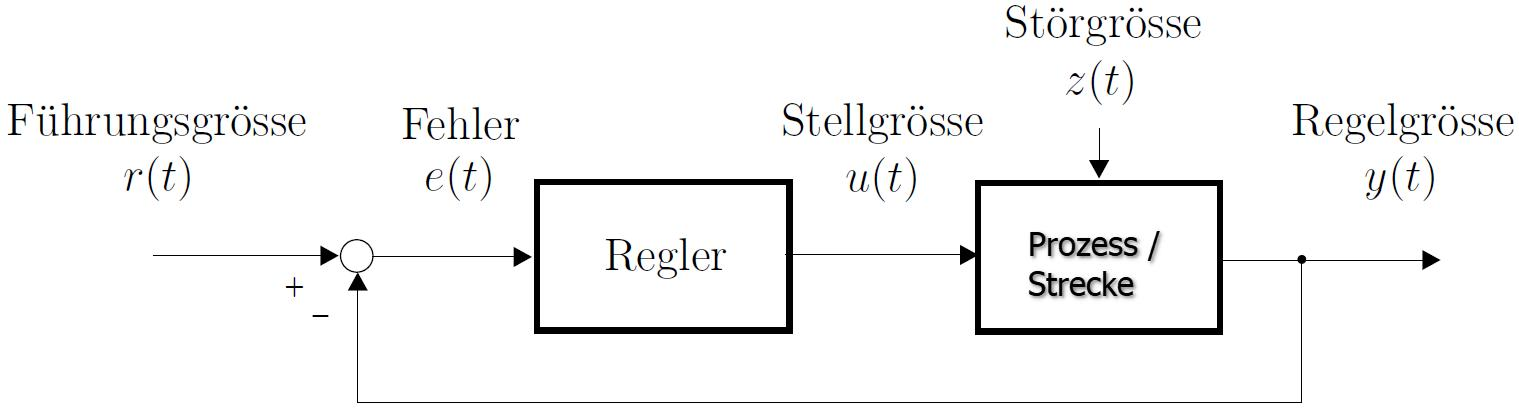
\includegraphics[width=0.85\columnwidth]{images/groessen_regelkreis.jpg}

	\vspace{0.2cm}

	\begin{tabular}{ l  l }
		\toprule
		Führungsgrösse $r(t)$ (Referenz)	& Gibt Sollwert vor 				\\
		\midrule
		Regelgrösse $y(t)$ 					& Zu regelnde Grösse 				\\
		\midrule
		Fehler $e(t)$ 						& Differenz $r(t) - y(t)$ 			\\
		\midrule
		Stellgrösse $u(t)$ 					& Regelerausgang / Streckeneingang	\\
		\midrule
		Störgrösse $z(t)$ (oder $d(t)$) 	& Störungen aller Art 				\\
		\bottomrule
	\end{tabular}
\end{center}


\subsection{Komponenten des Regelkreises}{16-17}

\begin{center}
	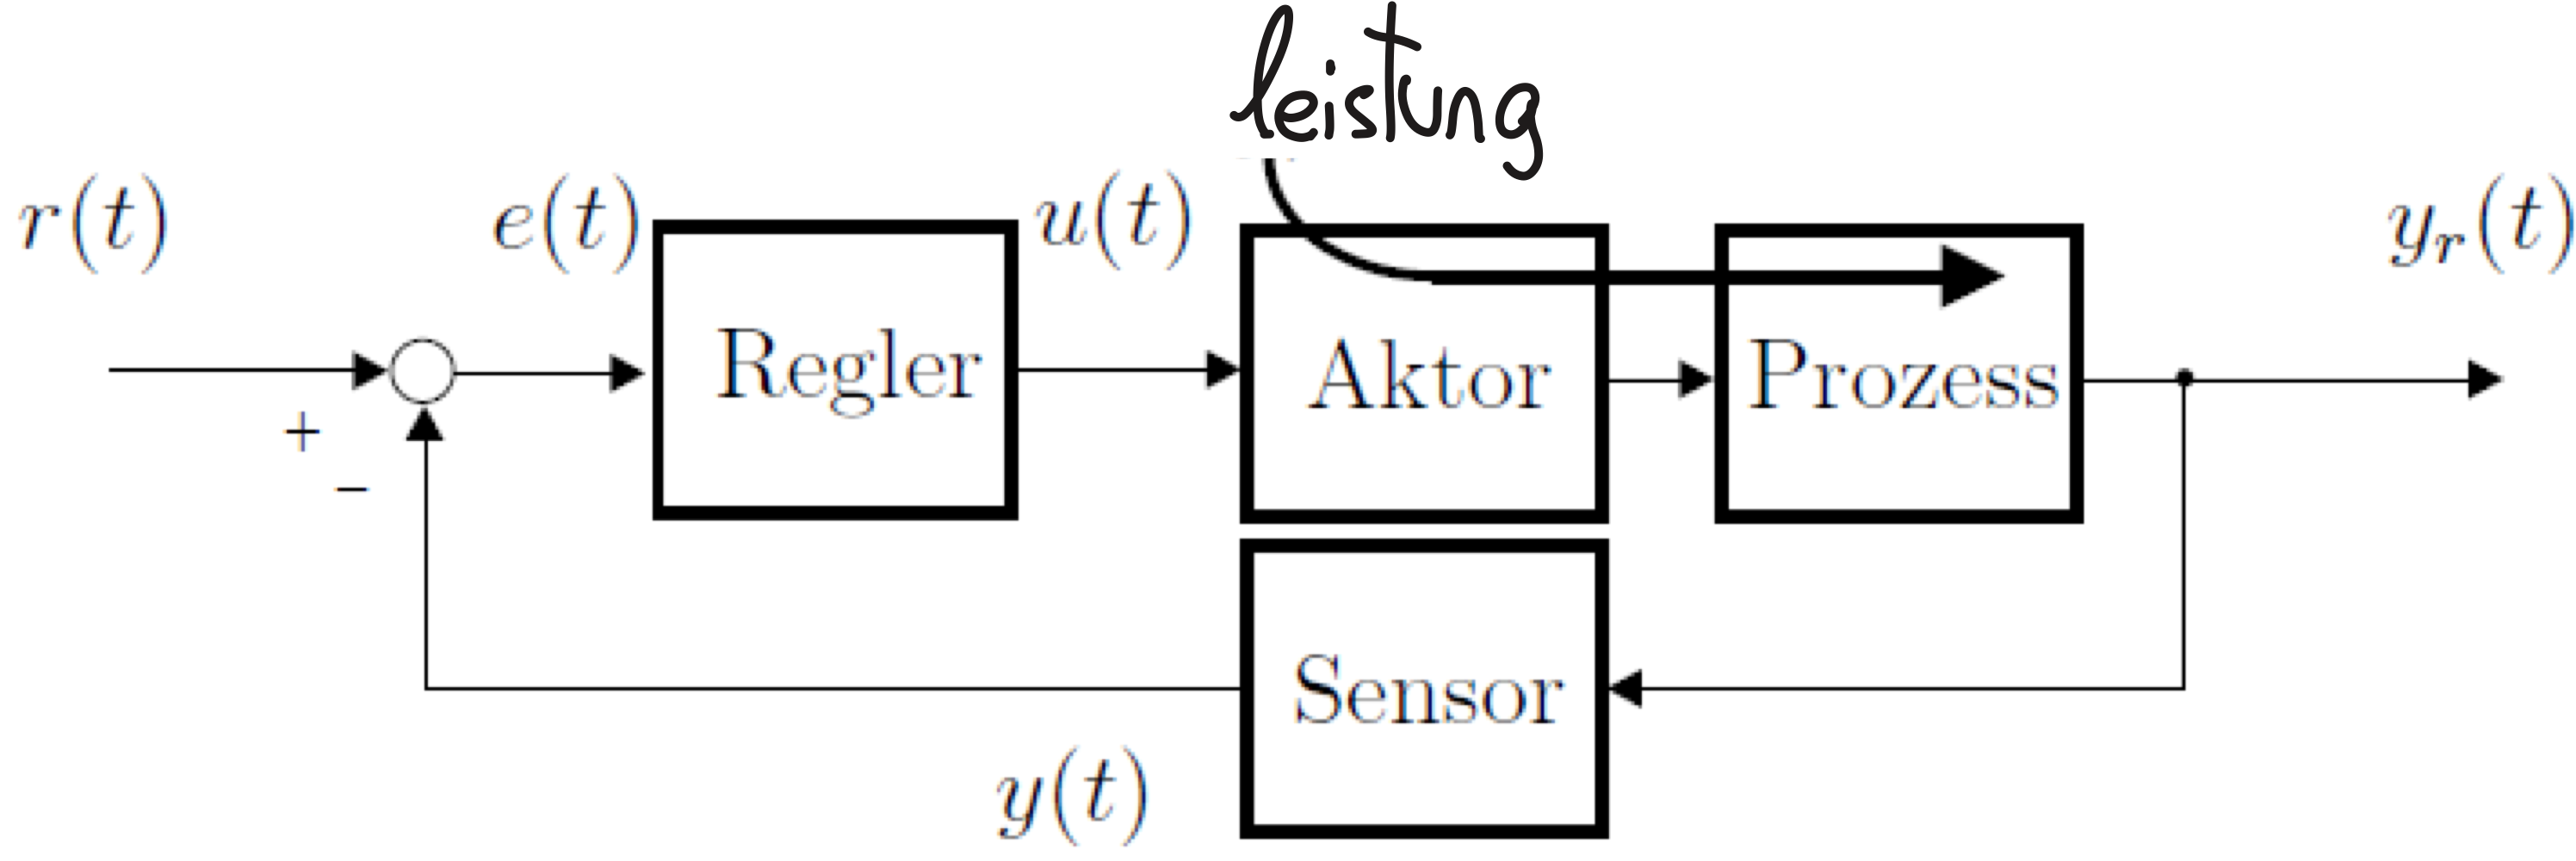
\includegraphics[width=0.8\columnwidth]{images/reglerkreis.png}
\end{center}


\begin{itemize}
	\item \textbf{Genauigkeit beim Sensor wichtiger als beim Aktor!}
	\item Leistung liefert Aktor (Stellglied) 
\end{itemize}


\subsection{Steuerung vs. Regelung}{18-19}

Die Steuerungstechnik liefert oft die Führungsgrösse für geregelte Untersysteme.

\textbf{Eine Regelung hat Feedback bzgl. der Referenz, eine Steuerung nicht!}

\begin{center}
	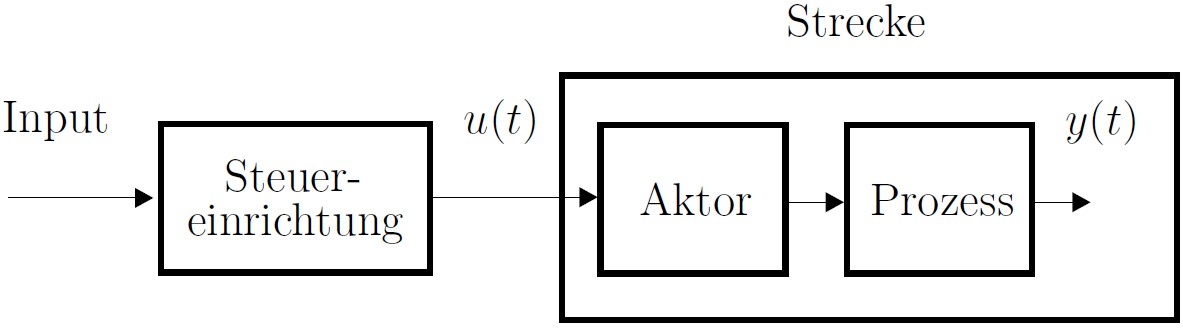
\includegraphics[width=0.8\columnwidth]{images/steuerung.jpg} 
\end{center}


\subsection{Prozess, System, Modell}{20}

\subsubsection{Prozess}
Gesamtheit zusammenwirkender Vorgänge, durch die Materie, Energie und Information umgeformt, transportiert und gespeichert wird.

\textrightarrow\ z.B. Fahren eines Autos (abstrakt)


\subsubsection{System}

Ist gegenüber der Umwelt abgegrenzt, hat Eingänge, Ausgänge (und Zustand).


\subsubsection{Modell}

Beschreibung von Systemen (häufig mit Hilfe der Mathematik)


\subsection{Modellierung}{21}

\begin{itemize}
	\item Ein Modell beschreibt \textbf{gewisse Aspekte} eines Prozesses
	\item Ein Modell beschreibt ein System \textbf{so genau wie nötig}
	\item \textbf{Alle Modelle sind falsch}
	\item Ein Modell muss an die Anwendung angepasst sein
\end{itemize}

\vspace{0.2cm}

Modellieren bedeutet, Systeme systematisch

\vspace{0.1cm}
\begin{itemize}
	\item in Teilsysteme zu teilen (Top-Down)
	\item aus Grundgliedern aufzubauen (Bottom-Up)
\end{itemize}

\columnbreak


\subsection{Beschreibungsmethoden von Systemen}

Alle genannten Methoden beschreiben ein System vollständig!

\vspace{0.2cm}

\begin{minipage}[t]{0.6\columnwidth}
	\raggedright

	\begin{itemize}
		\item Funktion oder LUT (statische Systeme)
		\item Sprungantwort (LZI-Systeme)
		\item Impulsantwort (auf Dirac-Stoss) 
		\item Übertragungsfunktion
		\item Frequenzgang
	\end{itemize}
\end{minipage}
\hfill
\begin{minipage}[t]{0.38\columnwidth}
	\raggedright

	\begin{itemize}
		\item Differenzialgleichungen
		\item Zustandsraum
		\item Block-Diagramm
		\item Bode-Diagramm
		\item Nyquist-Diagramm
		\item Pol-Nullstellen-Diagramm
	\end{itemize}
\end{minipage}


		\section{Statische Grundglieder (ohne Gedächtnis)}

Der Ausgang des Systems ist \textbf{nur} vom aktuellen Eingang abhängig 
$$ y(t) = f( u(t) ) $$
\cbl{\textbf{Hinweis:} $u(t)$ entspricht meist $A \cdot \varepsilon(t)$ (skalierter Einheitssprung)\label{u(t)}}


\subsection{P-Glied (Proportional)}{26}

$$ \boxed{ y(t) = K \cdot u(t) } $$

\begin{minipage}{0.23\columnwidth}
    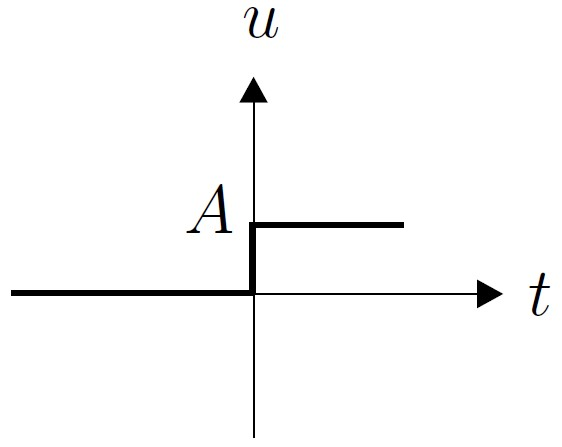
\includegraphics[width=0.8\columnwidth]{images/eingangssignal_schrittantwort.jpg} 
\end{minipage}
\hfill
    \begin{minipage}{0.23\columnwidth}
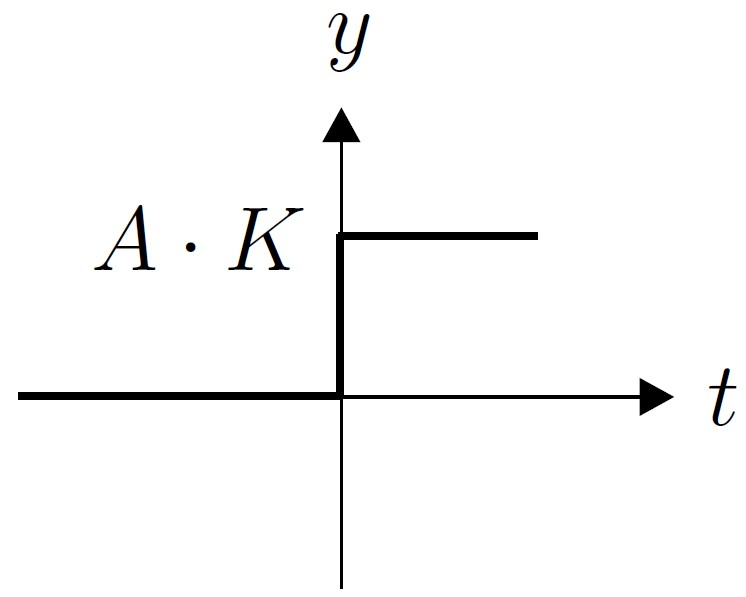
\includegraphics[width=0.8\columnwidth]{images/schrittantwort_p-glied.jpg} 
\end{minipage}
\hfill
\begin{minipage}{0.23\columnwidth}
    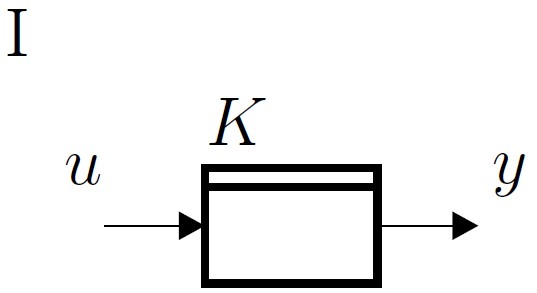
\includegraphics[width=0.8\columnwidth]{images/symbol_p-glied_1.jpg}
\end{minipage}
\hfill
\begin{minipage}{0.23\columnwidth}
    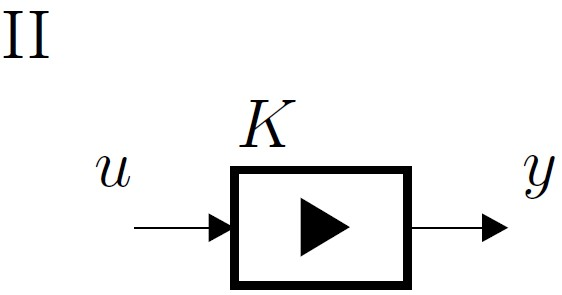
\includegraphics[width=0.8\columnwidth]{images/symbol_p-glied_2.jpg}
\end{minipage}


\subsection{Kennlinie / Pseudostatische Kennlinie}

\begin{minipage}[t]{0.25\columnwidth}
    \begin{center}
        \subsubsection{Kennlinie}

        \vspace{-0.4cm}
        $$ \boxed{ y(t) = f(u) } $$
        
        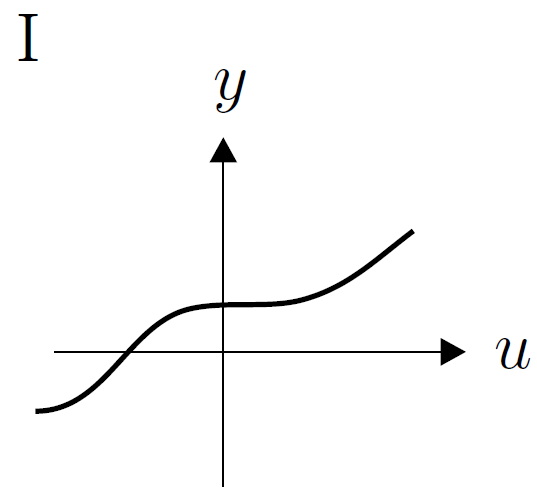
\includegraphics[width=0.85\columnwidth]{images/kennlinie.png}
    \end{center}
\end{minipage}
\hfill
\begin{minipage}[t]{0.7\columnwidth}
    \begin{center}
        \subsubsection{Pseudostatische Kennlinien}
        
        \vspace{-0.4cm}
        $$ \boxed{\text{Nicht mathematisch beschreibbar} }$$

        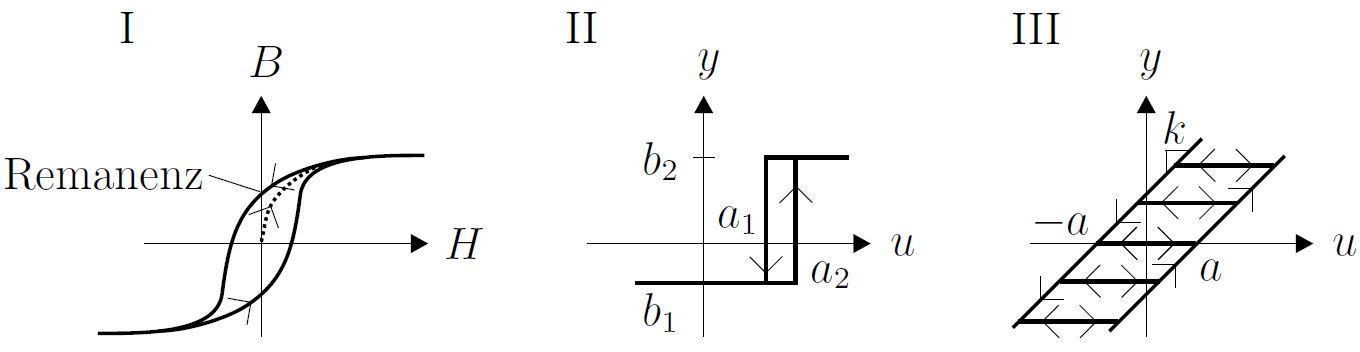
\includegraphics[width=\columnwidth]{images/pseudokennlinien.png}
    \end{center}
\end{minipage}


		\section{Dynamische Grundglieder (mit Gedächtnis)}

Der Ausgang des Systems ist vom aktuellen \textbf{und} von vergangenen Eingängen abhängig.
Vergangene Eingänge werden im System in einem Speicher, einem Zustand $x(t)$ abgelegt 
$$ y(t) = f( u(t), \, x(t) ) $$


\subsubsection{Prozesse mit / ohne Ausgleich}

\begin{tabular}{ll}
ohne Ausgleich: & Sprungantwort wächst grenzenlos an ($\to \infty$)                    \\
mit Ausgleich:  & Sprungantwort strebt gegen endlichen Wert             \\
				& \textrightarrow\ \textbf{Gegenkopplung} am Ausgang {\small(oder reibung, energieverlust, \dots)} 
\end{tabular}


\subsection{Totzeit-Glied}{30}

\vspace{-0.2cm}
$$ \boxed{ y(t) =  u(t - T_t) } $$

\begin{center}
    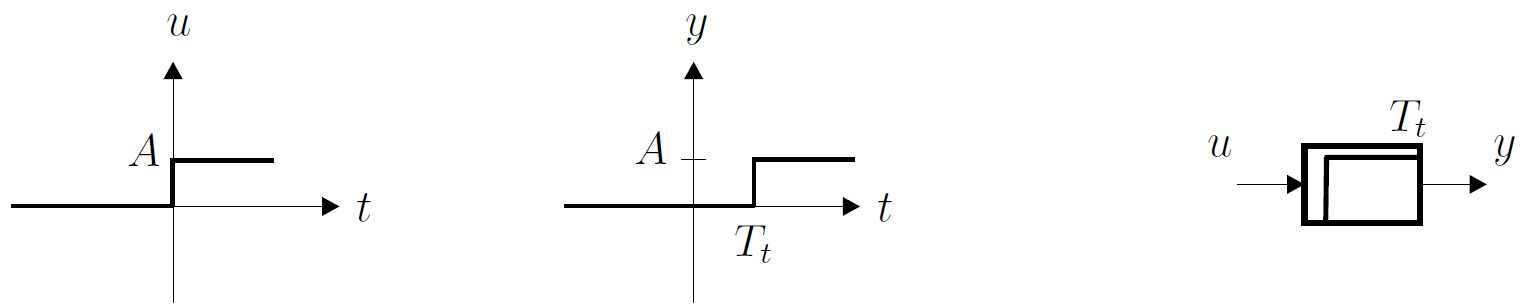
\includegraphics[width=0.9\columnwidth]{images/totzeit-glied.jpg}
\end{center}


\subsection{I-Glied (Integrierer)}{29}

\vspace{-0.3cm}
\begin{minipage}[c]{0.48\columnwidth}
    $$ \boxed{ \text{DGL:} \quad \dot{y}(t) = K \cdot u(t) }  $$
\end{minipage}
\hfill
\begin{minipage}[c]{0.48\columnwidth}
    $$ \boxed{ y = \int\limits_{- \infty}^t u(\tau) \, d \tau = K \int\limits_{- \infty}^t u(\tau) \, \diff \tau + y(0) } $$
\end{minipage}\vspace{-1em}

\begin{center}
    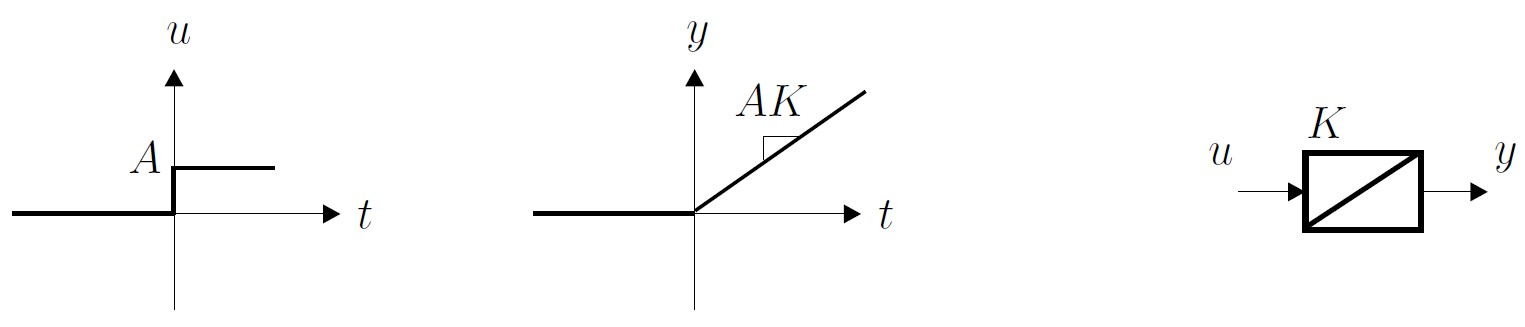
\includegraphics[width=0.9\columnwidth]{images/i-glied.jpg} 
\end{center}

\columnbreak


\subsection[PT1-Glied]{$\text{PT}_1$-Glied}{31-33}

Ein Energiespeicher \textrightarrow\ System schwingt \textbf{nicht}

\begin{minipage}[t]{0.48\columnwidth}
    $$ \boxed{ \text{DGL:} \quad  T \, \dot{y}(t) + y(t) = K \cdot u(t) }  $$
\end{minipage}
\hfill
\begin{minipage}[t]{0.48\columnwidth}
    $$ \boxed{ y(t) = K \, A + (y_0 - K \, A) \cdot e^{- \frac{t}{T}} } $$
\end{minipage}


\begin{minipage}{0.5\columnwidth}
    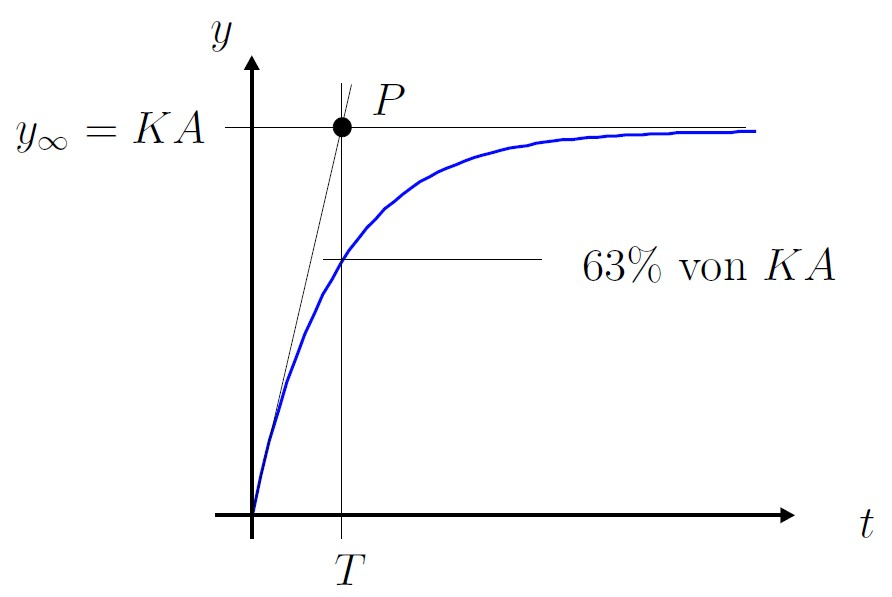
\includegraphics[width=\columnwidth]{images/pt1-glied_kennlinie.jpg}
\end{minipage}
\hfill
\begin{minipage}{0.4\columnwidth}
    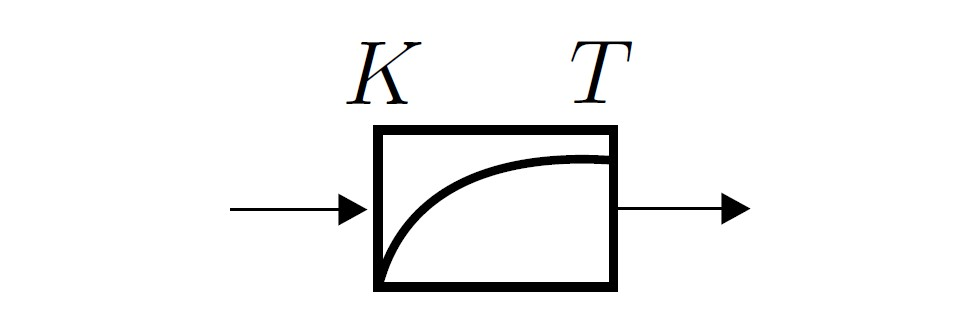
\includegraphics[width=0.8\columnwidth]{images/symbol_PT1-glied.jpg}
\end{minipage}


\subsubsection{Modellierung einer $\text{PT}_1$ Regelstrecke}

\begin{enumerate}
    \item Ausmessen der \hyperref[u(t)]{Sprungantwort} $u(t) = A \cdot \varepsilon(t)$ \\
        \textrightarrow\ Die Sprungantwort entspricht dem Diagramm
    \item  Parameter $K$ berechnen: $K = \dfrac{y_\infty - y_0}{A} = \dfrac{\Delta y}{A}$ \\
        \textit{(falls $u$ und $y$ nicht bei $0$ starten: $A = u_\infty - u_0$ und $\Delta y = y_\infty - y_0$ verwenden)}
    \item Parameter $T$ bestimmen: Tangente am Anfang durch Punkt $P = (t_0 + T_t,\, y_0)$ \\
    oder: Zeit bis $y(t) = y_0 + 0.63 \cdot \Delta y$ erreicht ist, \textbf{gemessen ab $t_0 + T_t$} \textrightarrow\ $T$ ablesen \\
    \textit{(Antwort mit Verzögerung $T_t$: $T = t_{63\%} - t_0 - T_t$)}
\end{enumerate}


\example{$\text{PT}_1$-Glied als Blockschaltbild}

\begin{minipage}[c]{0.48\columnwidth}
    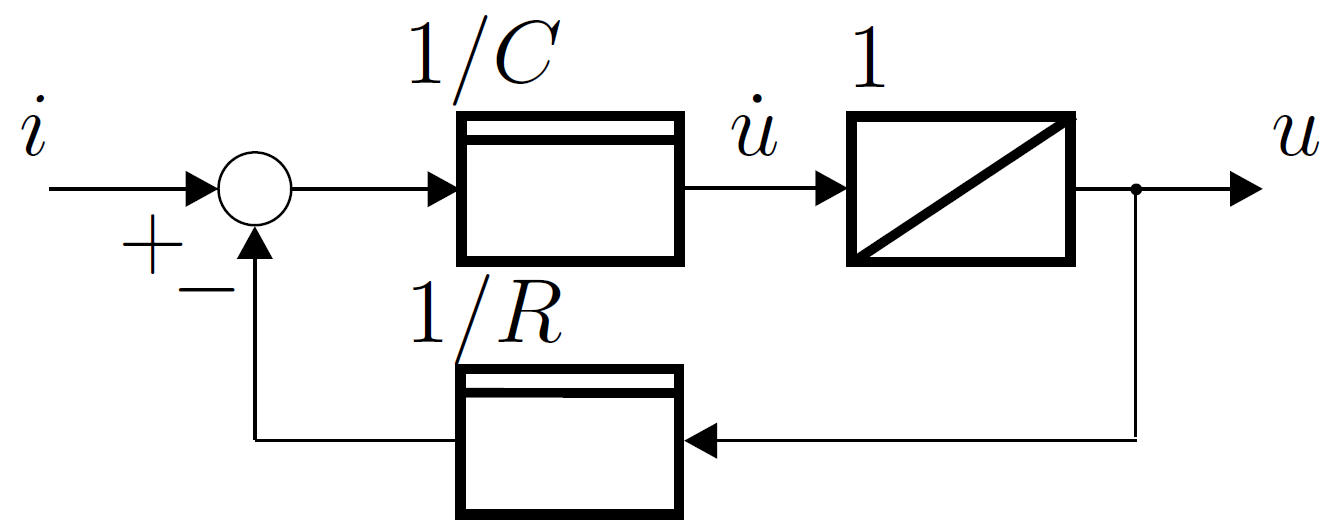
\includegraphics[width=\columnwidth]{images/pT1_blockschaltbild.png}
\end{minipage}
\hfill
\begin{minipage}[c]{0.48\columnwidth}
    $$ \boxed{ \text{Allg: } T \, \dot{y}(t) + y(t) = K \cdot u(t) } $$
    $$ \boxed{ \text{Bsp: } RC \, \dot{u}(t) + u(t) = R \cdot i(t) } $$
\end{minipage}


\subsection[PT2-Glied]{$\text{PT}_2$-Glied}{34}

Zwei Energiespeicher \textrightarrow\ \textbf{System kann schwingen}

\vspace{-0.2cm}

\begin{minipage}[c]{0.46\columnwidth}
    $$ \boxed{\text{DGL:} \quad T^2 \cdot  \ddot{y} + 2 \, \zeta \, T \cdot \dot{y} + y = K \cdot u } $$
\end{minipage}
\hfill
\begin{minipage}[c]{0.52\columnwidth}
    $$ \boxed{ y(t) = K \: A \Big[ 1 + e^{\sigma t} \big( - \cos(\omega t) + \frac{\sigma}{\omega} \sin(\omega t)  \big)  \Big] }  $$
\end{minipage}


\begin{minipage}{0.55\columnwidth}
    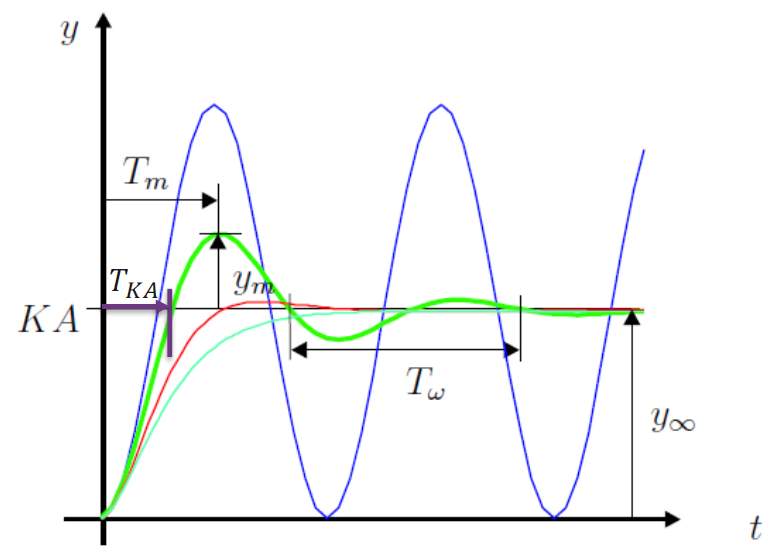
\includegraphics[width=\columnwidth]{images/pT2_sprungantwort.png}
\end{minipage}
\hfill
\begin{minipage}{0.38\columnwidth}
    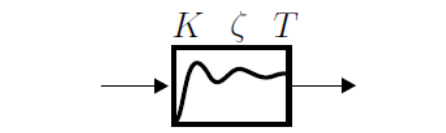
\includegraphics[width=0.75\columnwidth]{images/pT2_symbol.png}

    $$\omega = \omega_n \cdot \sqrt{1 - \zeta^2} $$
    $$ y_m = e^h \cdot y_{\infty} $$ 
\end{minipage}\vspace{-1em}


\begin{center}
    \renewcommand{\arraystretch}{1.8}
    \begin{tabular}{c c c}
        $K = \frac{y_{\infty}}{A}$                                      & $h = \ln \big( \frac{y_m}{y_{\infty}} \big)$                                  & $\omega = \frac{2 \, \pi}{T_{\omega}} = \frac{\pi}{T_m}$  \\
        $\sigma = \frac{h \, \omega}{\pi} = - \omega_n \cdot \zeta$     & $\omega_n = \sqrt{\omega^2 + \sigma^2} = - \frac{\sigma}{\zeta}$              & $\zeta = - \frac{h}{\sqrt{h^2 + \pi^2}}$                  \\
        $T = \frac{1}{\omega_n}$                                        & $T_{KA} = T_M - \frac{1}{\omega} \arctan \big(  \frac{\omega}{\sigma} \big)$  & $y(T_{KA}) = K \: A$
    \end{tabular}
    \renewcommand{\arraystretch}{1}
\end{center}

Il parametro $\zeta$ controlla la dämpfung (dämpfung alta \textrightarrow reazione lenta): 

\begin{tabularx}{\columnwidth}{XX}
    $\zeta = 0$: {\color{blue}Ungedämpft}&
    $\zeta = 1$: {\color{cyan}Ohne überschwingung}
\end{tabularx}

\subsection{D-Glied (Idealer Differenzierer)}{37}

\vspace{-0.2cm}
$$ \boxed{  y(t) = K \cdot \frac{\diff \, u(t)}{\diff t} = K  \cdot \dot{u}(t) } $$

\begin{minipage}{0.25\columnwidth} 
    \begin{center}
        \textbf{ideal}\\
        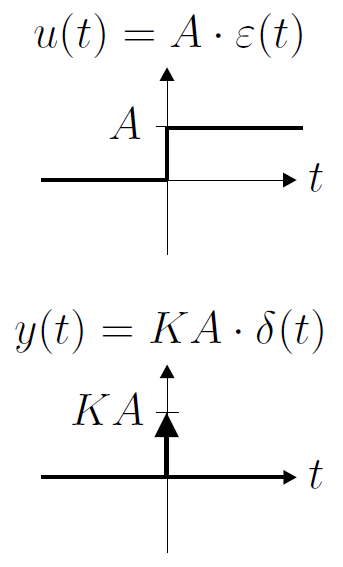
\includegraphics[width=0.9\columnwidth]{images/D-glied_ideal.png}
    \end{center}
\end{minipage}
\hfill
\begin{minipage}{0.25\columnwidth}
    \begin{center}
        \textbf{real}\\
        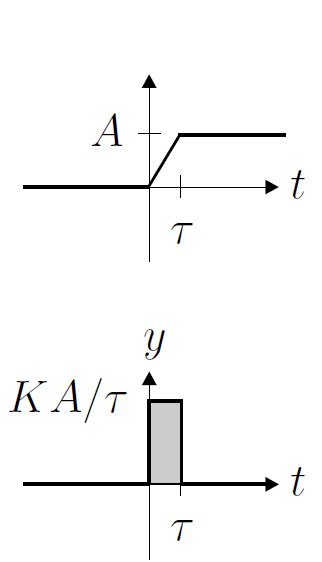
\includegraphics[width=0.9\columnwidth]{images/D-glied_real.png}
    \end{center}
\end{minipage}
\hfill
\begin{minipage}{0.25\columnwidth}
    \begin{center}
        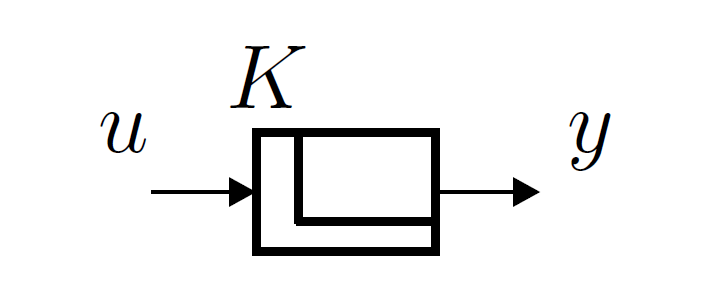
\includegraphics[width=0.9\columnwidth]{images/D-glied_symbol.png}
    \end{center}
\end{minipage}


\subsection[DT1-Glied (Realisierbarer Differenzierer)]{$\text{DT}_1$-Glied (Realisierbarer Differenzierer)}{38}

L'ordine dei blocchi è indifferente (prima derivatore o prima $\text{PT}_1$)

\begin{minipage}[c]{0.48\columnwidth}
    $$ \boxed{ w(t) = A \cdot (1 - e^{-\frac{t}{T}}) } $$
\end{minipage}
\hfill
\begin{minipage}[c]{0.48\columnwidth}
    $$ \boxed{ y(t) = \frac{K \cdot A}{T} \,  e^{-\frac{t}{T}} } $$
\end{minipage}

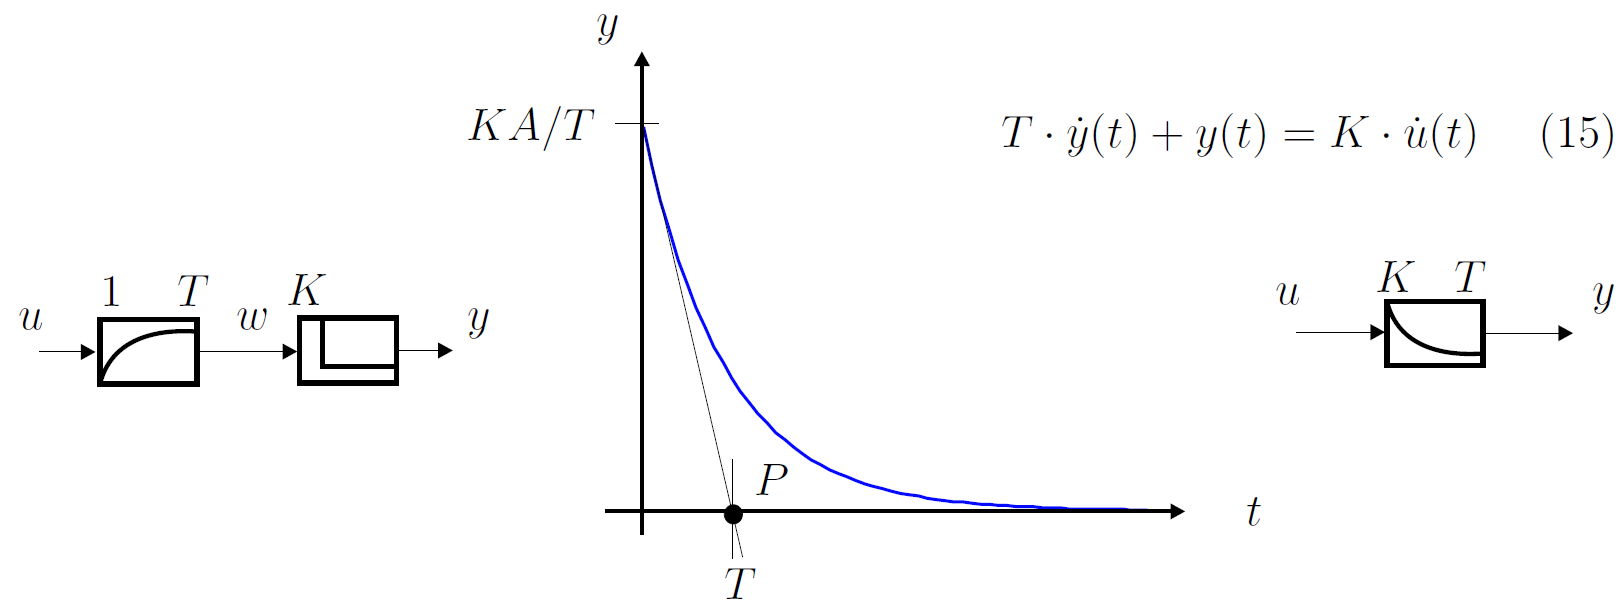
\includegraphics[width=\columnwidth]{images/DT1-glied.png}\vspace{-1em}


\example{Mögliche Realisierungen von $\text{DT}_1$-Gliedern}

\begin{minipage}[t]{0.48\columnwidth}
    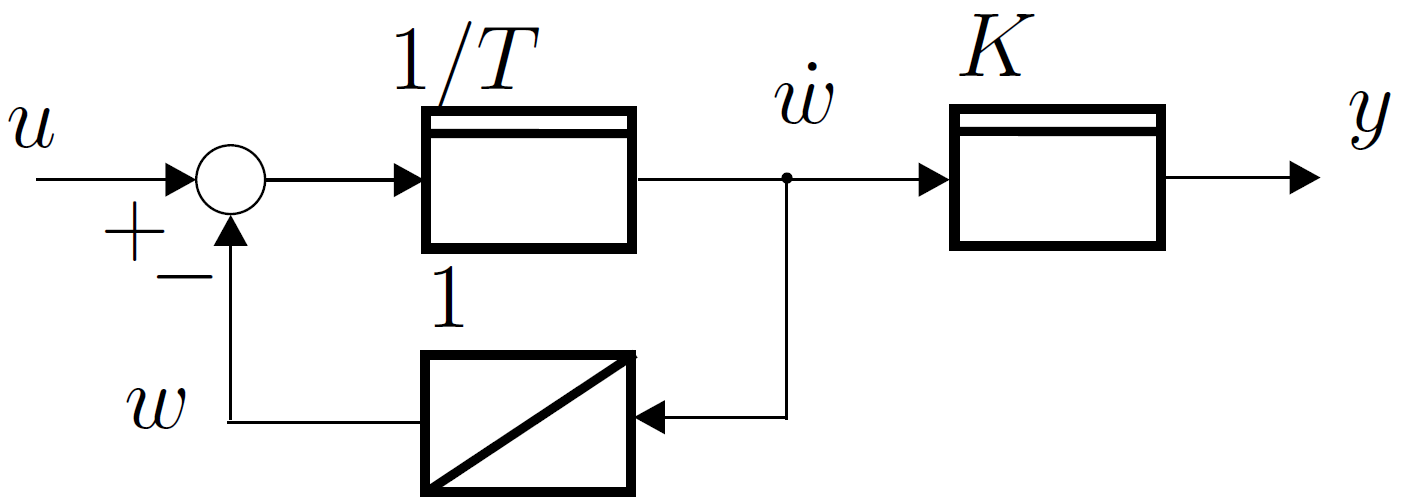
\includegraphics[width=\columnwidth, align=t]{images/pT1_blockschaltbild_2.png}
\end{minipage}
\hfill
\begin{minipage}[t]{0.48\columnwidth}
    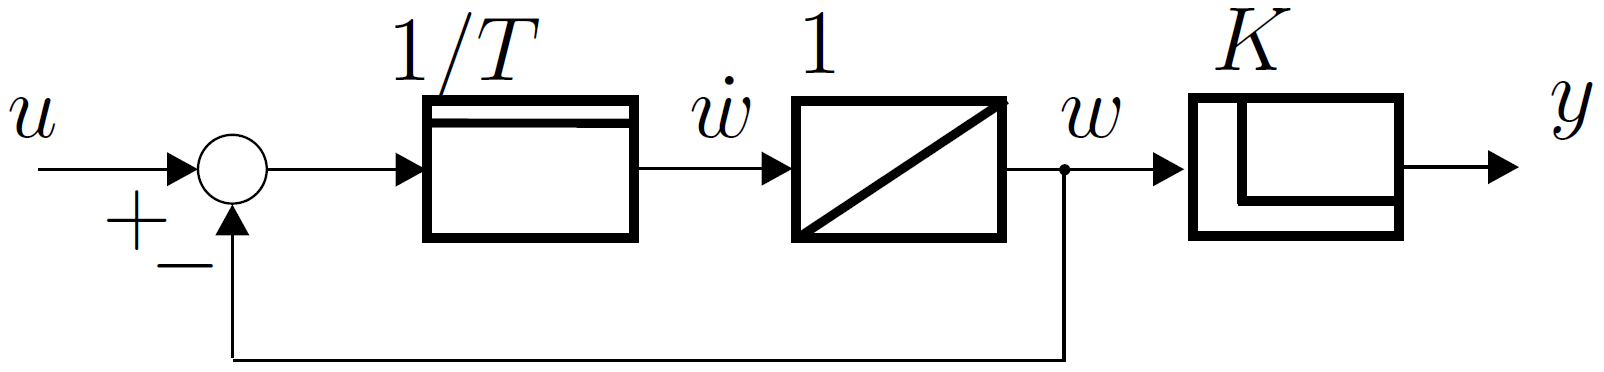
\includegraphics[width=\columnwidth, align=t]{images/DT1-glied_blockschaltbild.png}
\end{minipage}


\subsection{PID-Glied}{39}

\textbf{Zusammensetzen der Grundglieder: Parallelschaltung!} \\
Gilt auch für P, PI, PD, $\text{PDT}_1$ und $\text{PIDT}_1$ Glieder 
$$ \boxed{  y(t) = A \cdot \big[ K_P + K_I \cdot t + \frac{K_D}{T_C} e^{-\frac{t}{T_c}} \big]  }$$

\begin{minipage}{0.48\columnwidth}
    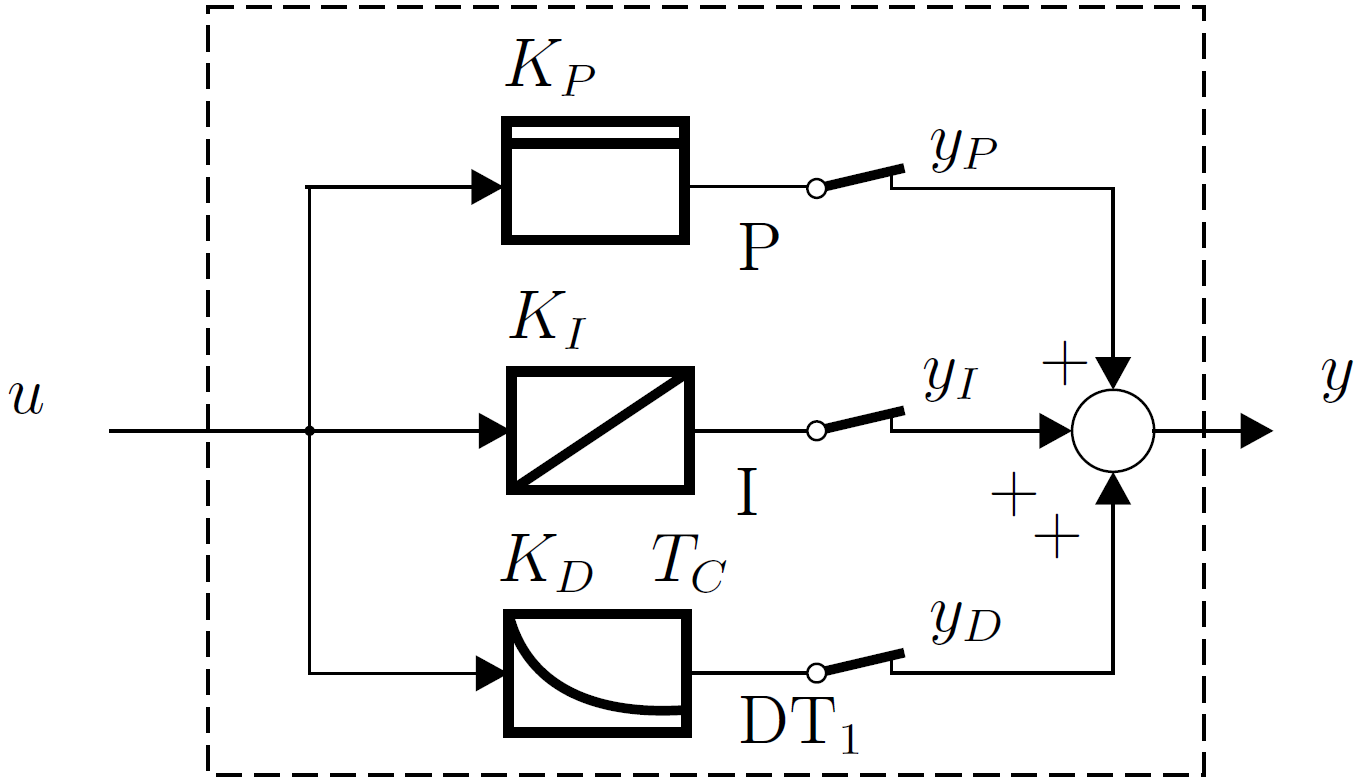
\includegraphics[width=0.9\columnwidth]{images/PID-glied.png}
\end{minipage}
\hfill
\begin{minipage}{0.5\columnwidth}
    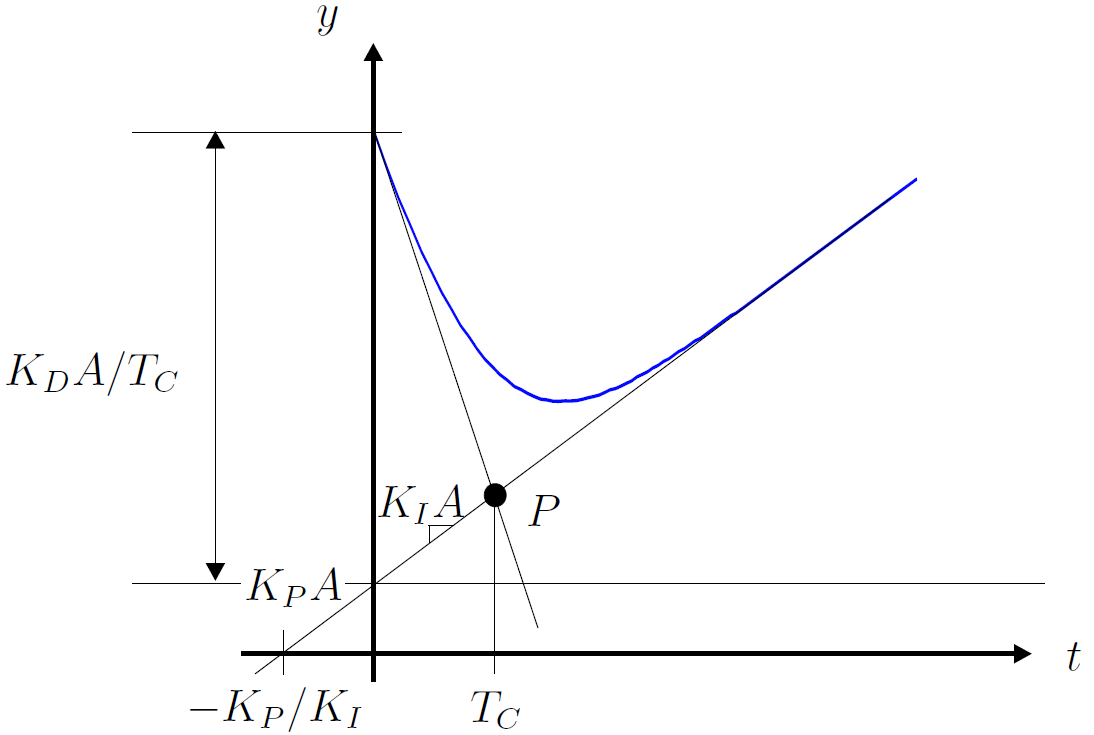
\includegraphics[width=\columnwidth]{images/PID_sprungantwort.png}
\end{minipage}


\subsection{Lead-Glied / Lag-Glied / Lead-Lag-Glied (S.40-41)}{40-41}

Lead-/ Lag-Glieder sind zwei Varianten von $\text{PDT}_1$-Gliedern. 

\vspace{0.2cm}
\begin{tabular}{ll}
    Lead:   & $K_P$ und $K_D$ haben \myul{gleiches} Vorzeichen          \\
    Lag:    & $K_P$ und $K_D$ haben \myul{unterschiedliches} Vorzeichen
\end{tabular}

\vspace{0.2cm}

Lead- und Lag-Glieder können auch als Parallelschaltungen eines P- und eines $\text{PT}_1$-Glieds aufgefasst werden. 

Das Lead-Lag-Glied  ist eine Serieschaltung aus Lead- und Lag-Glied.

\vspace{0.2cm}

\begin{minipage}{0.44\columnwidth}
    \begin{center}
        \textbf{Lead-Glied} \\
        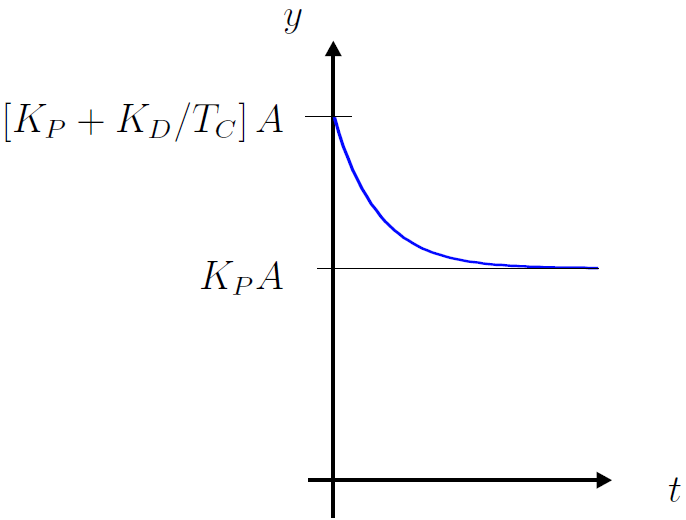
\includegraphics[width=\columnwidth]{images/lead-glied.png} 
    \end{center}
\end{minipage}
\hfill
\begin{minipage}{0.45\columnwidth}
    \begin{center}
        \textbf{Lag-Glied} \\
        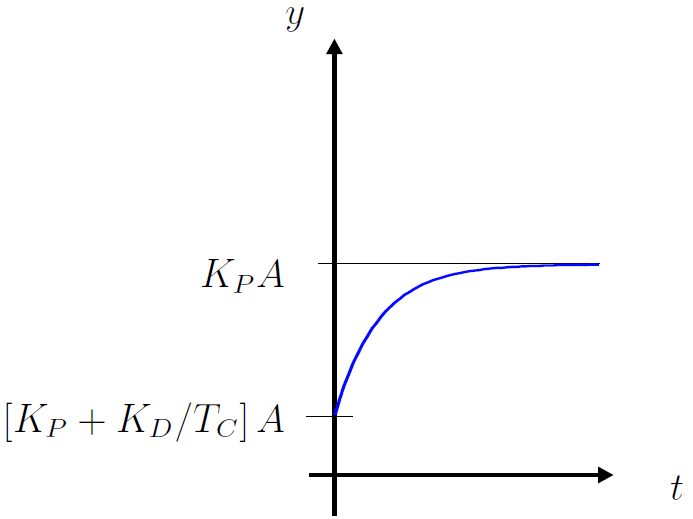
\includegraphics[width=\columnwidth]{images/lag-glied.png}
    \end{center}
\end{minipage}


		\section{Modellierung von Regelstrecken}{42}

\subsection{Vorgehen Modellierung von Regelstrecken}

\begin{enumerate}
  \item Identificare i singoli componenti del sistema
  \item Modellare ogni componente come elemento base (\textit{Grundglied})
  \item Scrivere la DGL del sistema tramite un bilancio (forze, portata, energia/calore, \dots)
  \begin{itemize}
    \item Sostituire passo per passo i componenti uno nell'altro
    \item In forma normale PT1/PT2 \cbl{la grandezza di interesse $y(t)$ deve comparire senza coefficiente}
  \end{itemize}
  \item Dalla DGL disegnare lo schema a blocchi con gli elementi base
  \begin{itemize}
    \item Isolare derivata più alta, disegnare integratori, disegnare P-Glied e connettere ($+ / -$)
    \item Servono tanti integratori (\textit{I-Glieder}) quanto è l'ordine della DGL
  \end{itemize}
\end{enumerate}


\example{Modellierung von Regelstrecke}{43}

\begin{minipage}[c]{0.45\columnwidth}
    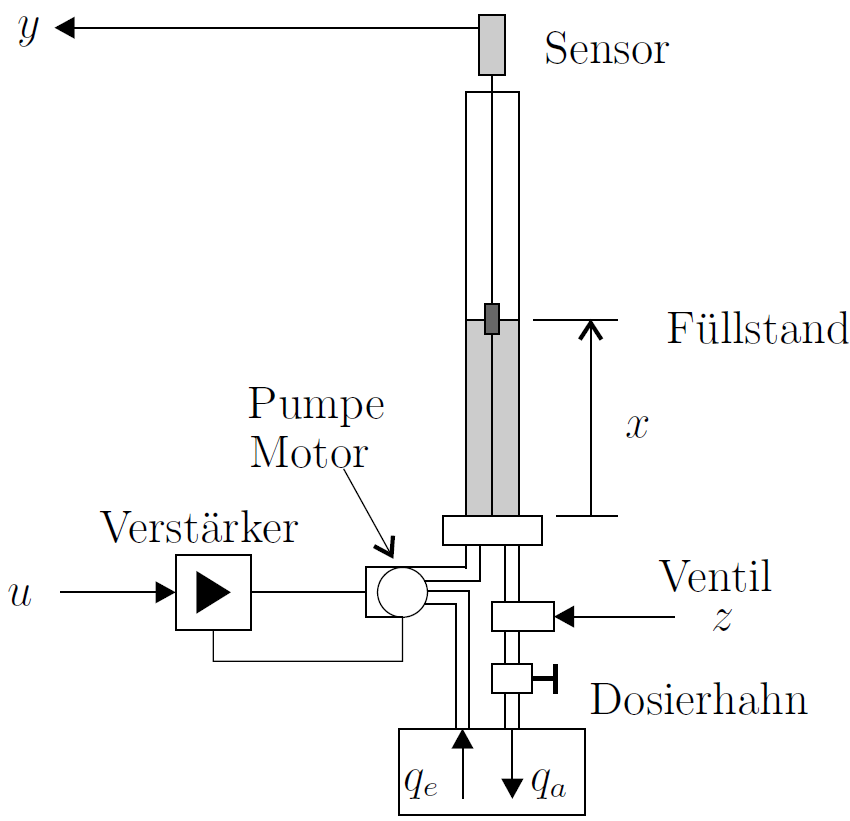
\includegraphics[width=\columnwidth]{images/modellierung_fuellprozess.png}
\end{minipage}
\hfill
\begin{minipage}[c]{0.5\columnwidth}
    \begin{enumerate}
        \setlength\itemsep{1em}

        \item \textbf{Pumpleistung $\bm{q_e}$} \\
            $q_e(t) = K_P \cdot u(t) \qquad [K_P] = \frac{\meter^3}{\volt \, \second}$

        \item \textbf{Fluss durch Ventil} \\
            \begin{minipage}[c]{0.5\columnwidth}
                $q_a(t) = \begin{cases}
                    0 & z = 0 \\
                    Q_a & z = 1 \end{cases}$
            \end{minipage}
            \hfill
            \begin{minipage}[c]{0.44\columnwidth}
                $q_a(t) = Q_a \cdot z$
            \end{minipage}

        \item \textbf{Füllstand} \\
            $\dot{x}(t) = \underbrace{ \frac{1}{A_{\phi}} }_{\substack{K_I}} (q_e(t) - q_a(t)) $

        \item \textbf{Messung $\bm{y}$} \\
            $y(t) = K_M \cdot x(t) \quad [K_M] = \frac{\volt}{\meter} $
    \end{enumerate}
\end{minipage}


\begin{minipage}[t]{0.48\columnwidth}
    \textbf{DGL aufstellen}
    \begin{align*}
        \dot{y} &= K_M \cdot \dot{x}                \\
        \dot{y} &= K_M \cdot K_I \cdot (q_e - q_a)  \\
        \dot{y} &= K_M \cdot K_I \cdot (K_P \cdot u - Q_a \cdot z)
    \end{align*}
\end{minipage}
\hfill
\begin{minipage}[t]{0.48\columnwidth}
    \textbf{Modell zeichnen} 

    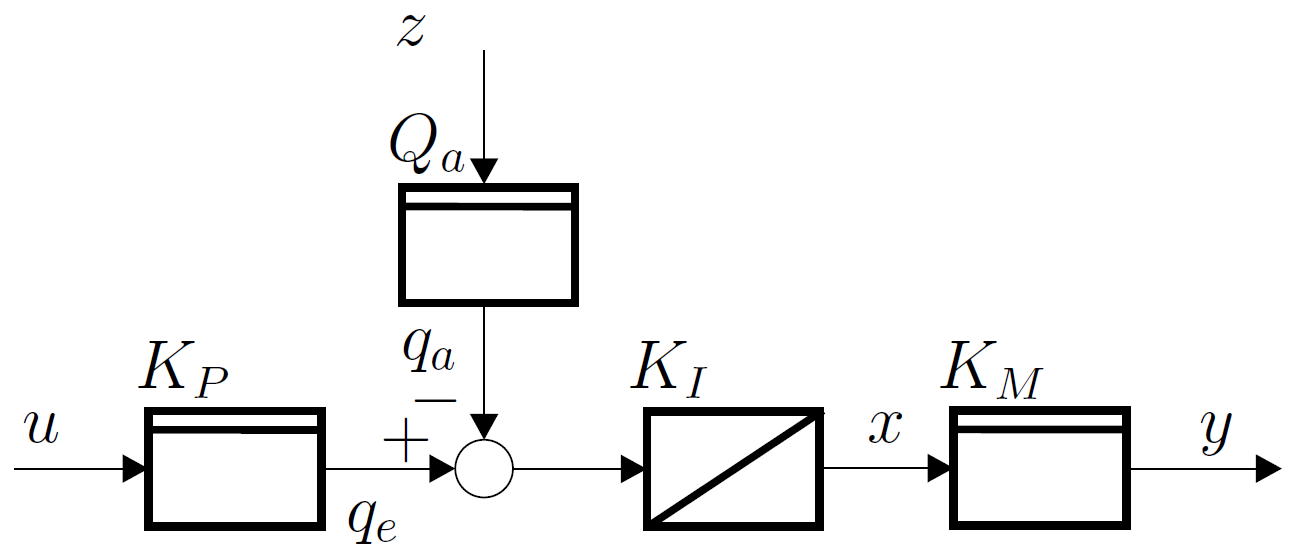
\includegraphics[width=\columnwidth]{images/modell_fuellprozess.png}
\end{minipage}


\vspace{0.2cm}

\textbf{Konstanten bestimmen} 

\begin{tabular}{ll}
    $K_M$   & Datenblatt                                                                    \\
    $K_I$   & Berechnung aus Geometrie                                                      \\
    $K_P$   & Parameter geschickt auf $0$ / bekannte Messgrössen setzen                     \\
            & $z=0, \, u(t) = A$ \quad \textrightarrow\ $\dot{y} = K_M \, K_P \, K_I \, A$  \\
    $Q_a$   & Parameter geschickt auf $0$ / bekannte Messgrössen setzen                     \\
            & $z=1, \, u(t) = 0$ \quad \textrightarrow\ $\dot{y} = - K_M \, K_I \, Q_a$
\end{tabular}


\subsubsection{Trick: Variablentransformation}

Wenn eine DGL ähnlich aussieht wie ein Grundglied (z.B. $\text{PT}_1$ oder $\text{PT}_2$), jedoch eine \textbf{Differenz von Variablen}
in der DGL vorkommt, wird die Variablentransformation angewendet.

\renewcommand{\arraystretch}{1.8}
\begin{tabular}{ll}
DGL:                                & $T \cdot \dot{y}(t) + [ \cor{y(t) - y_a(t)} ] = K \cdot u(t)$                 \\
Transformtaion:                     & $\Delta y = y - y_a \qquad \Delta \dot{y} = \dot{y} - \dot{y_a} = \dot{y}$    \\
DGL in $\text{PT}_1 \text{-Form}$:  & $T \cdot \Delta \dot{y}(t) + \cor{\Delta y(t)} = K \cdot u(t)$ 
\end{tabular}
\renewcommand{\arraystretch}{1}


\subsection{Vorgehen Blockdiagramm zu DGL}

\begin{itemize}
  \item Il numero di integratori corrisponde all'ordine della DGL
  \item Partire dal nodo sommatore prima del primo integratore ($\ddot{y} = \dots$)
  \item Etichettare le uscite degli integratori con $y, \dot{y}, \ddot{y}, \dots$ partendo dal lato dell'uscita
  \item Se la struttura lo permette, riscrivere la DGL nella forma dell'elemento PT1 o PT2 ($y$ senza vorfaktor)
\end{itemize}
		\section{Schaltende Regler}

\subsection{Klassifizierung von Regelstrecken oder Modellen}

\begin{itemize}
    \item statisch $\leftrightarrow$ \underline{dynamisch} 
    \begin{itemize}
        \item Drehzahlregelung eines Getriebes?
        \item Stromregelung eines Widerstandes?
    \end{itemize}
    \item akausal $\leftrightarrow$ \underline{kausal}
    \begin{itemize}
        \item Eine Strecke reagiert immer unmittelbar oder verzögert aber nie 'im Voraus' reagieren
        \item Ein Regler kann nicht verfrüht auf eine Störung
    \end{itemize}
    \item \underline{linear} $\leftrightarrow$ nichtlinear
    \item \underline{zeitinvariant} $\leftrightarrow$ zeitvariant
    \item \underline{mit Ausgleich} $\leftrightarrow$ ohne Ausgleich
    \item \underline{konzentrierte Parameter} $\leftrightarrow$ verteilte Parameter
    \begin{itemize}
        \item ODE vs. PDE
    \end{itemize}
    \item \underline{deterministisch} $\leftrightarrow$ stochastisch
    \begin{itemize}
        \item Führungsgrösse: Deterministisch
        \item Störgrösse: Stochastisch
    \end{itemize}
\end{itemize}


\subsection{Stetiger Regler vs. Schaltende Regler}

Ein \textbf{stetiger Regler} kann/soll auf \textbf{kleine Änderungen} der Signale reagieren \\
(z.B. 16 Bit A/D-Wandler) 

\vspace{0.2cm}

Einem \textbf{schaltenden Regler} stehen Signale nur in \textbf{beschränkter Auflösung} zur Verfügung - oft nur 1 Bit. 
Ein zu schnelles Hin- und Herschalten des Reglers wird oft durch eine \textbf{Hysterese} verhindert. 


\subsection{Zweipunktregler (Strecke: Integrator)}{64}

\vspace{-0.2cm}
$$ \boxed{\text{Fehler:} \quad e(t) = r(t) - y(t)} $$
\begin{center}
    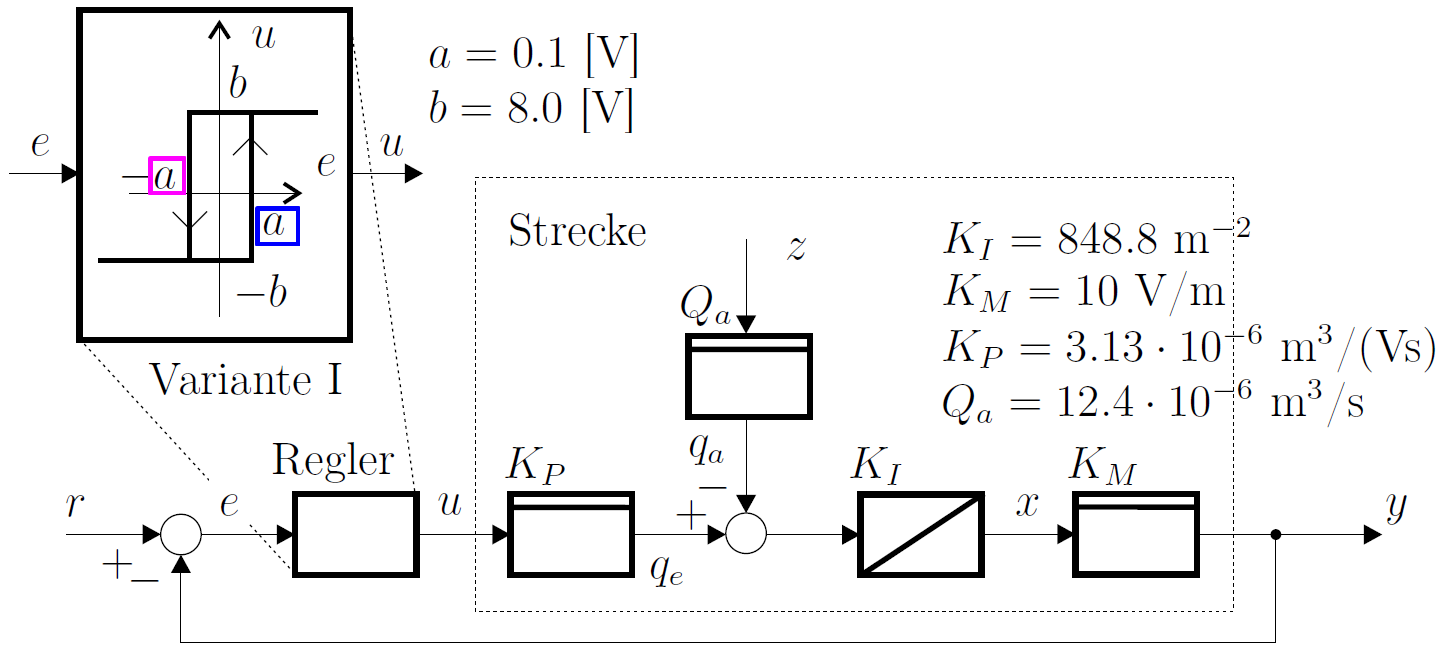
\includegraphics[width=0.85\columnwidth]{images/zweipunkteregler_beispiel.png} 
\end{center}


\subsubsection{Berechnungen am Grenzzyklus}{65-66}

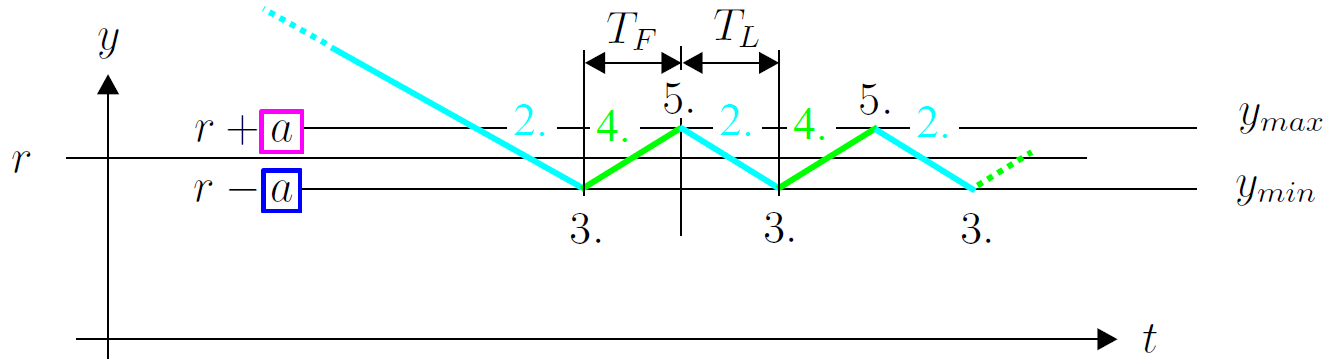
\includegraphics[width=\columnwidth]{images/grenzzyklus.png}

\fbox{\parbox{0.96\columnwidth}{
    \renewcommand{\arraystretch}{1.7}
    \begin{tabular}{ll}
        $y_{\rm max}$   & Maximalwert von $y$ während des Zyklus                                \\
        $y_{\rm min}$   & Minimalwert von $y$ während des Zyklus                                \\
        $\Delta y $     & $\Delta y = y_{\rm max} - y_{\rm min}$ \quad (Schwankungsbereich)     \\
        $y_m$           & $y_m = \frac{y_{\rm max} + y_{\rm min}}{2}$ \quad (Mittelwert)        \\
        $T$ 	        & Periodendauer des Grenzzyklus
    \end{tabular}  
    \renewcommand{\arraystretch}{1}

    $$ T = T_F + T_L = \frac{y_{\rm max} - y_{\rm min}}{K_M \, K_I \, K_P  \,b} + \frac{y_{\rm min} - y_{\rm max}}{- K_M \, K_I \, K_P  \,b} = \frac{4 \, a}{K_M \, K_I \, K_P  \,b} $$
} }
  
  

\subsection[Zweipunktregler (Strecke: PT1 mit Totzeit)]{Zweipunktregler (Strecke: $\text{PT}_1$ mit Totzeit)}{68}

\begin{minipage}[c]{0.65\columnwidth}
    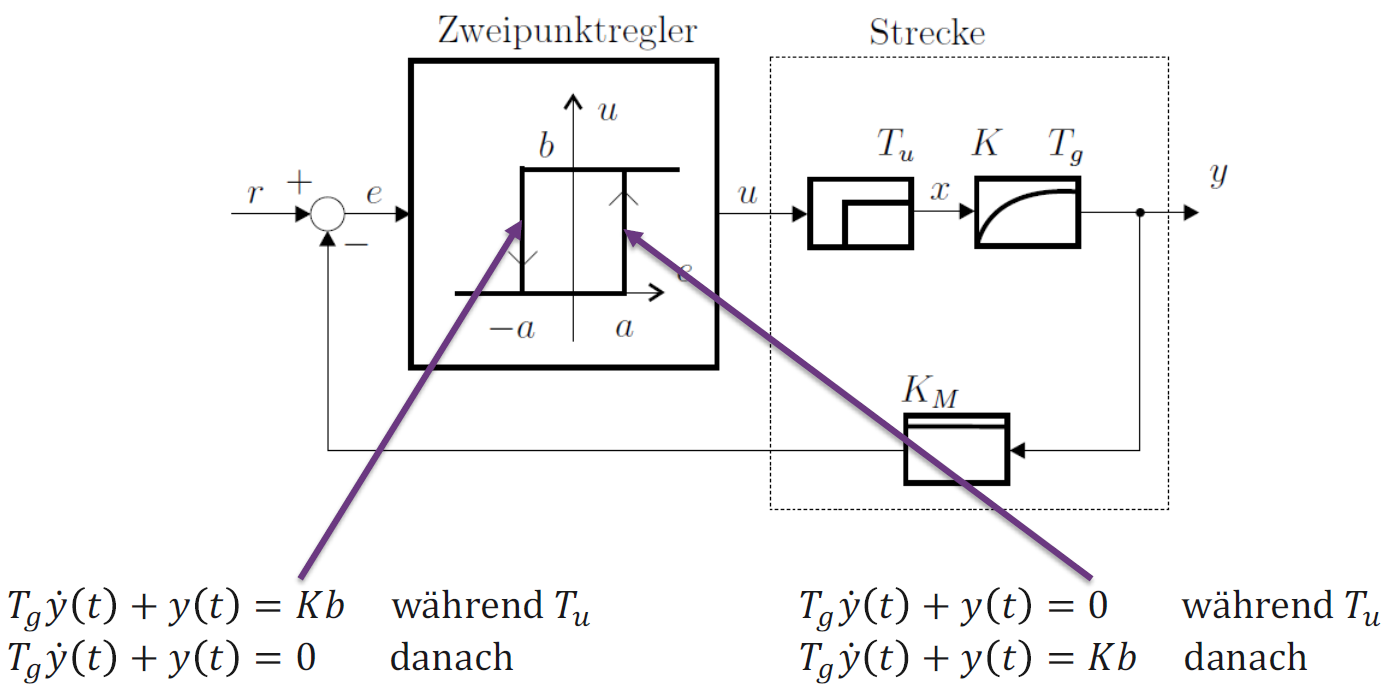
\includegraphics[width=\columnwidth]{images/zweipunkteregler_PT1.png}
\end{minipage}
\hfill
\begin{minipage}[c]{0.33\columnwidth}
    $$ \boxed{e(t) = r(t) - y(t) }$$
\end{minipage}

\begin{center}
    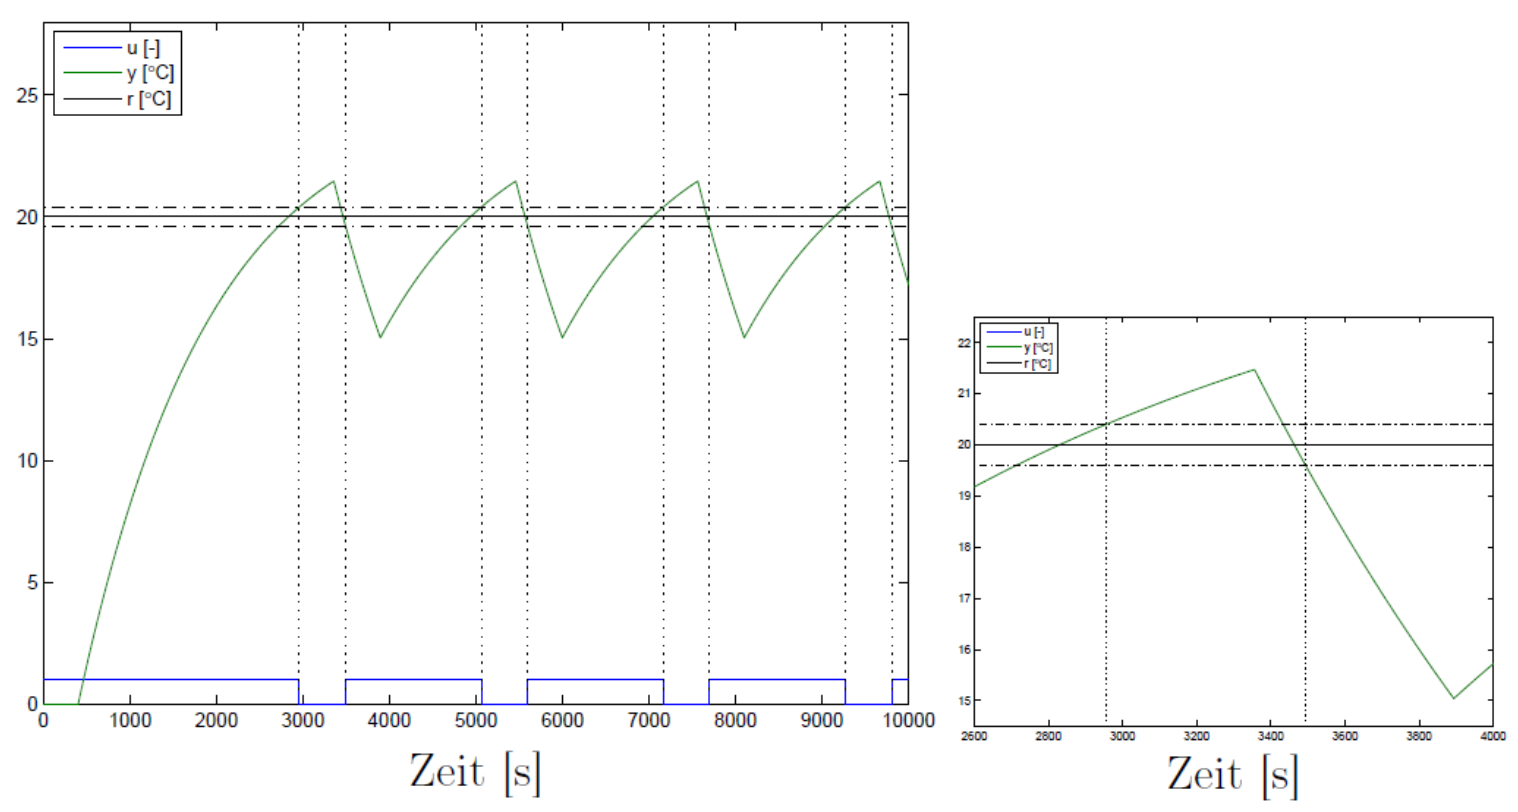
\includegraphics[width=0.9\columnwidth]{images/zweipunkteregler_PT1_simulation.png} 
\end{center}

\begin{enumerate}
    \item $y(t)$ wegen Totzeit nicht in Toleranzband $r \pm a$
    \item $y(t)$ ist im Mittel $y_m$ deutlich unterhalb von $r$
    \item Berechnungen werden viel aufwändiger
    \item Kennwerte ($y_m, \, T, \ ...$) sind von Amplitude abhängig 
\end{enumerate}


\subsubsection{Berechnungen am Grenzzyklus}

\begin{center}
    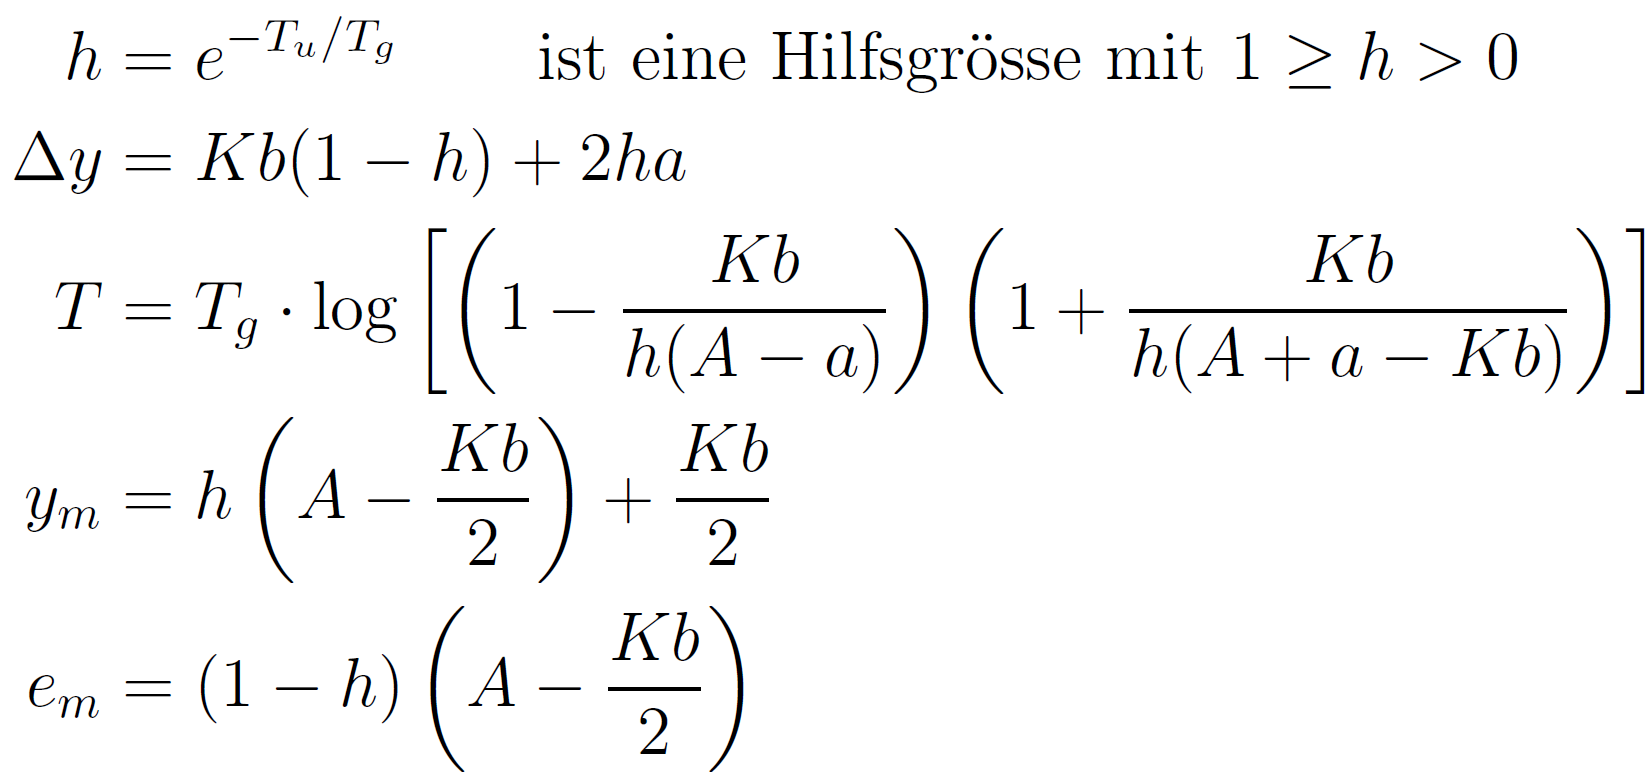
\includegraphics[width=0.7\columnwidth]{images/zweipunkteregler_PT1_berechnungen.png} 
\end{center}


\subsection{Dreipunkteregler / Mehrpunkteregler}{71}

\begin{minipage}[c]{0.3\columnwidth}
    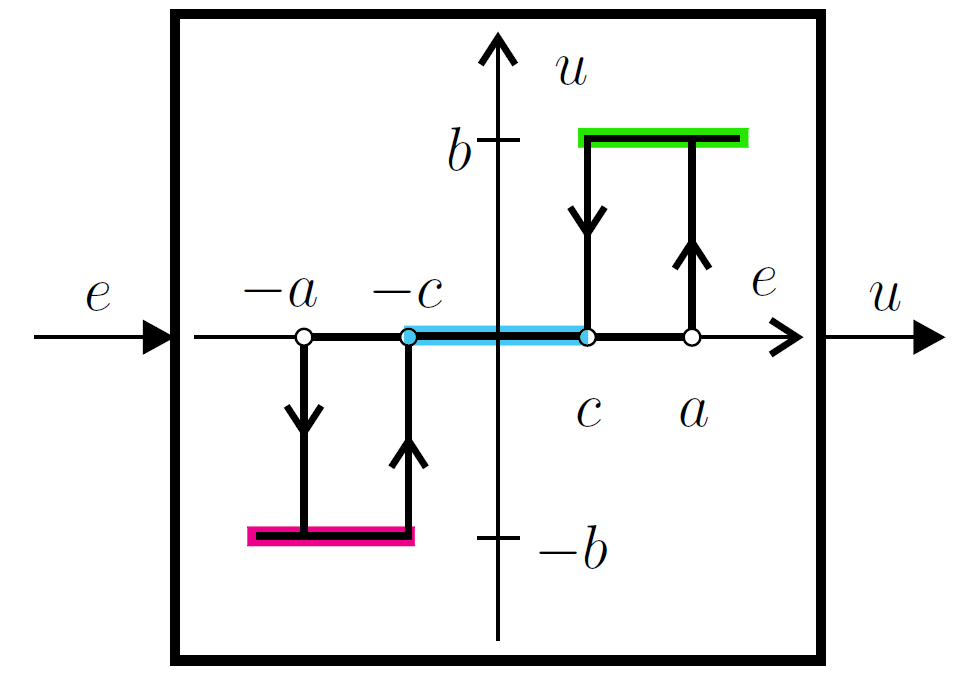
\includegraphics[width=\columnwidth]{images/dreipunkteregler.png}
\end{minipage}
\hfill
\begin{minipage}[c]{0.66\columnwidth}
    \raggedright
    Ein Dreipunkteregler hat drei mögliche Werte für das Stellsignal $u(t)$, z.B. vorwärts, aus und rückwärts. 
    Die Realisierung kann z.B. mit \textbf{zwei Hysteresen} erfolgen, wobei sich \textbf{vier Schaltbedingungen} ergeben. 
\end{minipage}


		\section{Stetigähnliche Regler}

Die Stellgrösse $u(t)$ ist noch immer auf wenige Werte beschränkt. \\
Mit den folgenden Konzepten (Abschnitt \ref{Zweipunkteregler mit interner Rückkopplung} und \ref{Schrittregler}) wird aber
erreicht, dass die \textbf{Strecke trotzdem mehr oder weniger 'stetig' beeinflusst} werden kann. \\
\textbf{Gegenüber schaltenden Reglern sind stetigähnliche Regler also aufwendiger zu bauen, aber am Regelausgang ändert sich nicht viel.}

\columnbreak


\subsection{Zweipunkteregler mit interner Rückkopplung}{72}

\label{Zweipunkteregler mit interner Rückkopplung}

\example{$\text{PT}_1$-Glied mit Totzeit als Strecke}

\textbf{Regelinterne Rückkopplung} ($\text{PT}_1$-Glied) zur Reduktion der Schwankungsbreite.
Dieses reagiert ähnlich wie die Strecke, allerdings schneller ($T_r$ klein) und weniger stark \\
($K_r$ gross)

\begin{center}
    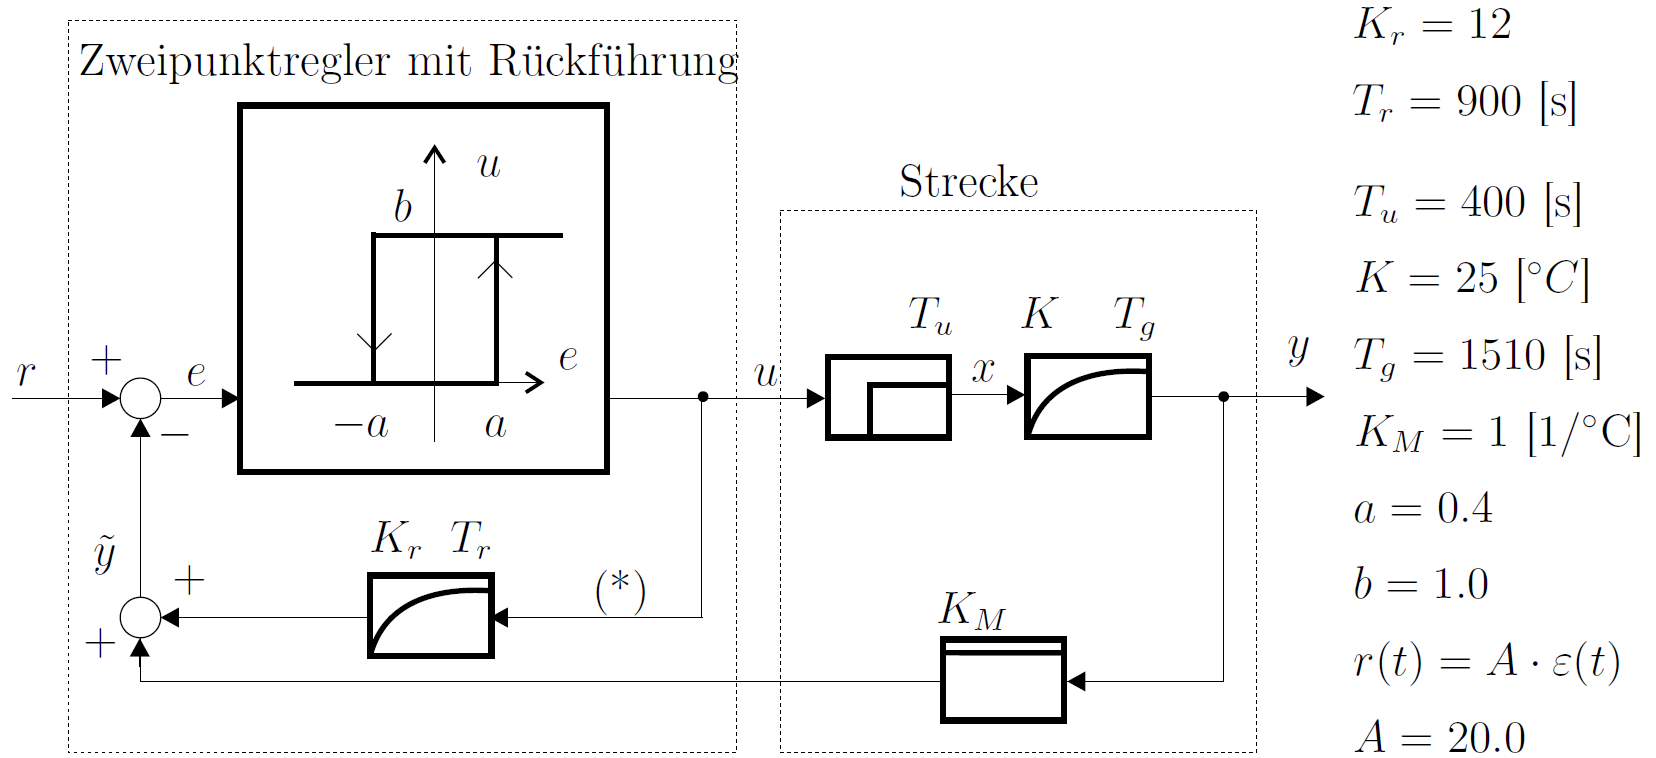
\includegraphics[width=0.8\columnwidth]{images/zweipunkteregler_mit_rueckfuehrung.png}
\end{center}


\textbf{Problem an dieser Schaltung:}

Die Schwankungsbreite ist zwar reduziert, jedoch wird der Sollwert gar nicht erreicht\\
($y_m$ zu tief) \\
Begründung: DC-Verstärkung durch Rückkopplung verändert: 
$$ \tilde{y}_{\rm stat} = (K_M + \frac{K_r}{K}) \cdot y_{\rm stat} \approx 1.5 \cdot y_{\rm stat} $$ 
\textrightarrow\ Dem Regler wird ein zu grosser Messwert geliefert!

\vspace{0.2cm}
\textbf{Alternative:} \\
An der Stelle (*) zusätzlich ein $\text{DT}_1$-Glied einfügen, damit dieser Pfad die DC-Verstärkung Null bekommt.


\subsection{Schrittregler}{74}
\label{Schrittregler}

Häufig befindet sich am Prozesseingang ein Stellantrieb
\vspace{0.1cm}

\textrightarrow\ Fiktive Stellgrösse $v$ kann jeden beliebigen Wert annehmen \\
\textrightarrow\ Regler eher stetig als schaltend 

\begin{center}
    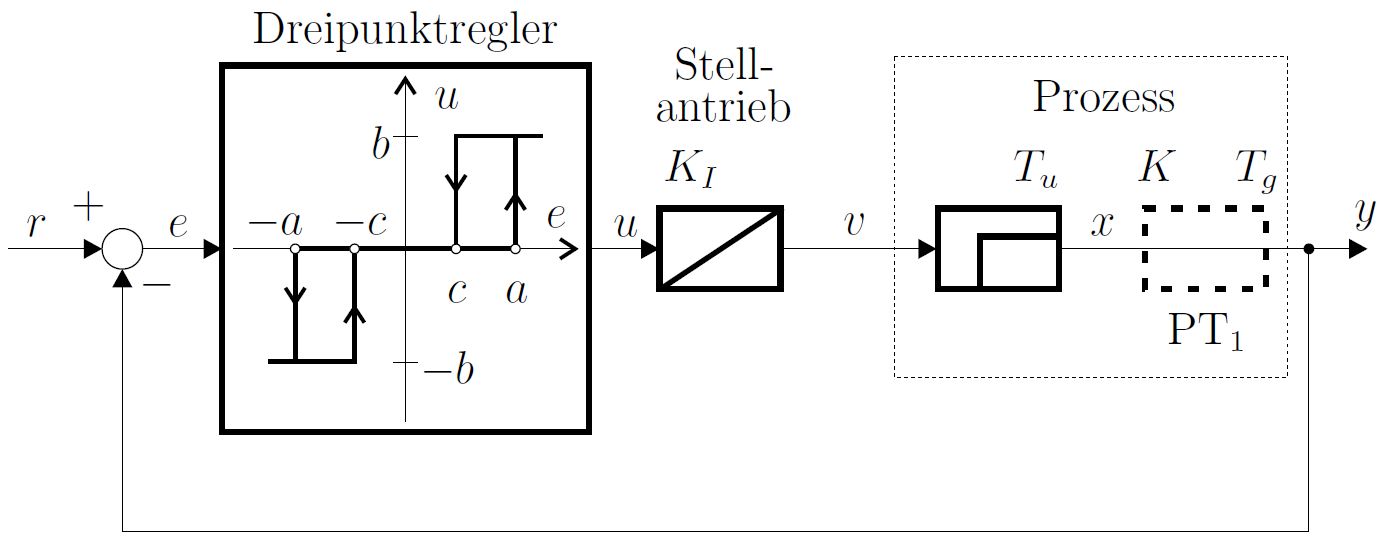
\includegraphics[width=0.8\columnwidth]{images/schrittregler.png}
\end{center}


\example{Stellglied und reiner Totzeit-Prozess (ohne $\text{PT}_1$-Glied)}

$u(t)$ darf nicht erst dann Null gesetzt werden, wenn $y = A$ erreicht wird, da der Prozess noch 'weiterläuft' (Totzeit)

\vspace{0.2cm}

\begin{minipage}{0.44\columnwidth}
    \begin{tabular}{ll}
        $u(t) = b$                      & für $A > a$   \\
        $r(t) = A $                     &               \\
        $v(t) = K_I \, \cdot b \cdot t$ 
    \end{tabular}
\end{minipage}
\hfill
\begin{minipage}{0.55\columnwidth}
    $y(t) =\begin{cases}
    0                               & \text{für } t < T_u   \\
    K_I \, \cdot b \cdot (t - T_u)  & \text{für } t \geq T_u
    \end{cases}$
\end{minipage}

\vspace{0.2cm}

\begin{minipage}{0.65\columnwidth}
    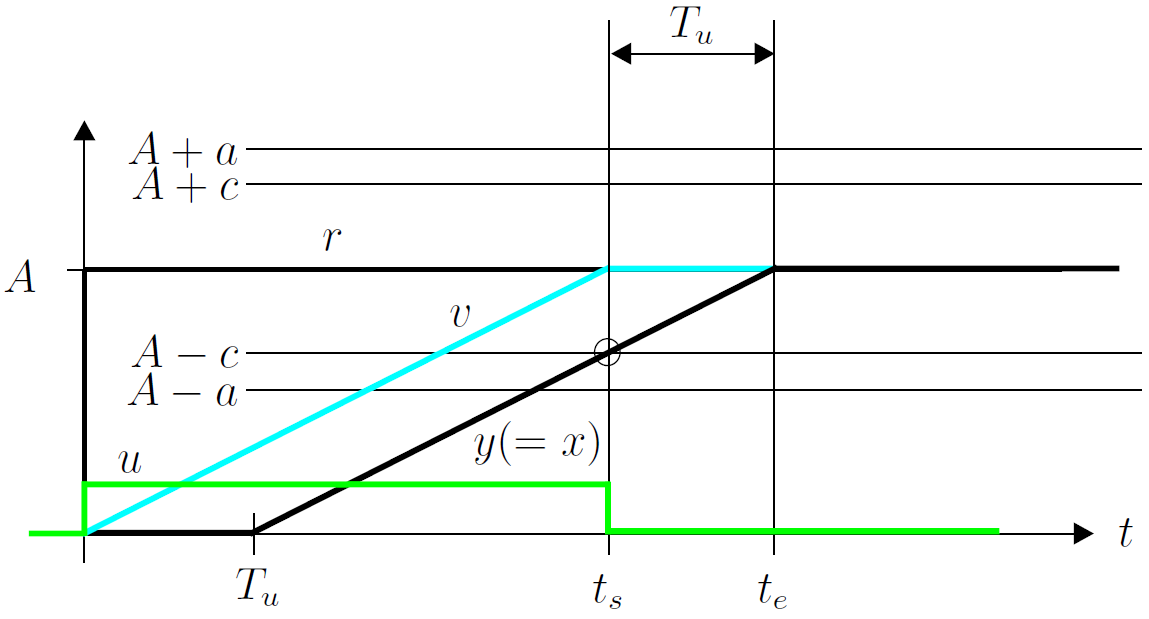
\includegraphics[width=0.9\columnwidth]{images/stellglied_nur_totzeit.png}
\end{minipage}
\hfill
\begin{minipage}{0.32\columnwidth}
    $$ t_e = \frac{A}{K_I \cdot B} + T_u $$
    $$ t_s = t_e - T_u = \frac{A}{K_I \cdot b} $$ 
\end{minipage}

\vspace{0.2cm}
\textbf{Ideale Abschaltzeit $\bm{t_s}$ durch Zurückrechnen finden:} 
$$ y(t_s) = K_I \cdot b \cdot (t - T_u) = A - K_I \cdot b \cdot T_u = A - c $$
$$ \underbrace{ K_I \cdot b}_{\substack{\text{Steigung}}} \cdot T_u = c $$

Parameter $b$ und $c$ auf einander abstimmen, um idealen Ausschaltzeitpunkt zu erreichen


		\section{Lineare Zeitinvariante Systeme (LZI)}

Für \textbf{lineare, zeitinvariante Systeme} gibt es viele Analyse- und Synthesemethoden für Regler \\
\textrightarrow\ Für \textbf{Entwurf} von Reglern gewünscht

\vspace{0.2cm}

Reale Systeme sind hingegen \textbf{nichtlinear und zeitvariant} \\
\textrightarrow\ Für \textbf{Simulation / Validierung} von Reglern gewünscht 


\subsection{Linearität (Definition)}{77}

Gegeben sei ein System 
$$ \Phi: u(t) \rightarrow y(t) \qquad y(t) = \Phi(u(t))$$
Wenn das System das \textbf{Superpositionsprinzip erfüllt}, so ist das System \textbf{linear} \\
\textrightarrow\ 'Es kommt nich auf die Reihenfolge der Operationen an'

$$ \boxed{ \cgn{ \Phi( \alpha_A \cdot u_A(t) + \alpha_B \cdot u_B(t)) } = \cbl{ \alpha_A \cdot \Phi(u_A(t)) + \alpha_B \cdot \Phi(u_B(t)) } } $$

\begin{center}
	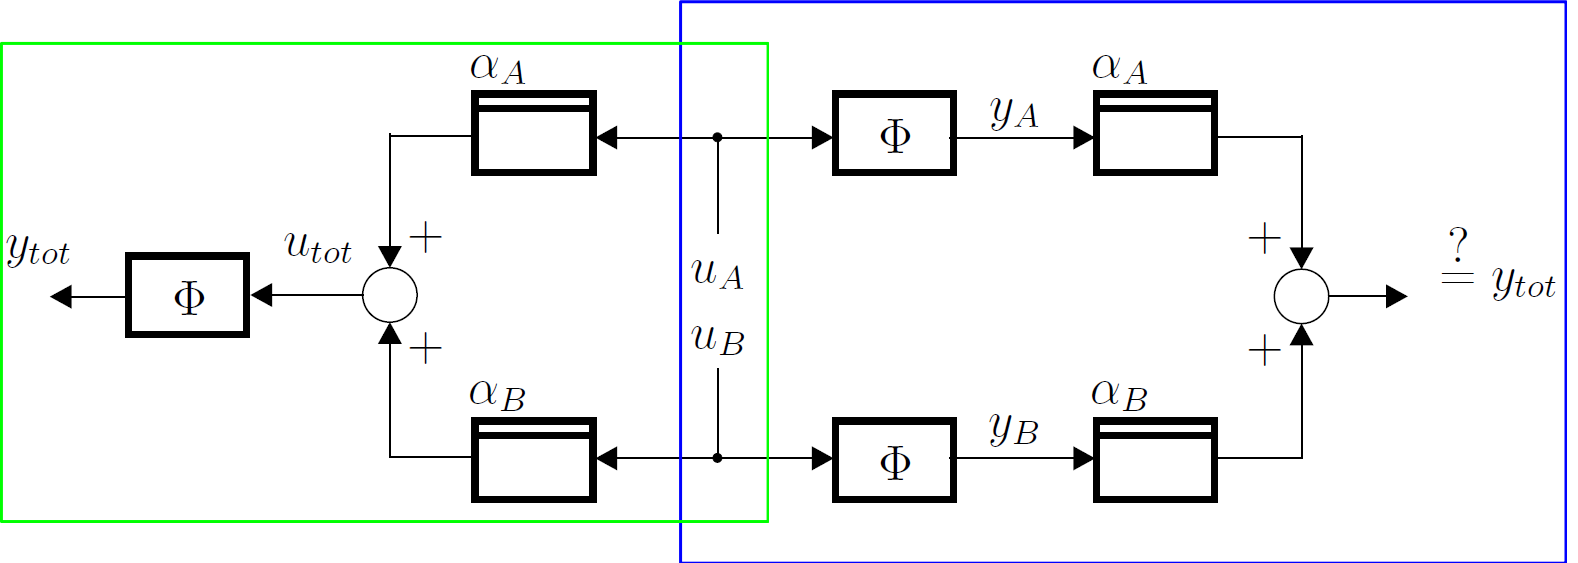
\includegraphics[width=0.9\columnwidth]{images/pruefung_linearitaet.png} 
\end{center}

Ein guter Test ist, ein \textbf{'Gegenbeweis'} mit der Bedingung $u(t) = 0$ 
$$ \Phi(0 \cdot u(t)) = 0 \cdot \Phi(u(t)) = 0 $$
\textrightarrow\ Wenn dieser Test \textbf{fehlschlägt} ist das System \textbf{nichtlinear}!


\subsection{Lineare Systeme}

Alle Systeme, die mit \textbf{Differentialgleichungen mit konstanten Koeffizienten} beschrieben werden, sind linear 
$$ \boxed{ a_n y(t)^{(n)} + ... + a_1 \dot{y}(t) + a_0 y(t) = b_m u(t)^{(m)} + ... + b_1 \dot{u}(t) + b_0 u(t) } $$
\textrightarrow\ Zeitverschiebung ändert nichts an der Linearität des Systems!


\subsubsection{Beispiele linearer Systeme}

\begin{minipage}[t]{0.4\columnwidth}
	\begin{tabular}{lll}
		\tabitem Verstärkung 			& $y(t) = K \cdot u(t)$ 					\\
		\tabitem Integrator 			& $\dot{y}(t) = u(t)$ 						
	\end{tabular}
\end{minipage}
\hfill
\begin{minipage}[t]{0.58\columnwidth}
	\begin{tabular}{lll}
		\tabitem Differenzierer 		& $y(t) = \dot{u}(t)$ 						\\
		\tabitem $\text{PT}_1$-Glied 	& $T \, \dot{y}(t) + y(t) = K \cdot u(t)$ 
	\end{tabular}
\end{minipage}


\subsection{Zeitinvarianz (Defintion)}{79}

Gegeben sei ein System 
$$\Phi: u(t) \rightarrow y(t) \qquad y(t) = \Phi(u(t))$$

Ist das System zeitinvariant, so gilt
$$ \boxed{ \Phi(u(t-T_t)) = y(t - T_t) \quad \forall \; T_t } $$
\textrightarrow\ Die Antwort des Systems ist unabhängig davon, zu welchem Zeitpunkt der Eingang anliegt


\subsubsection{Eigenschaften zeitvarianter Systeme}

\begin{itemize}
	\setlength\itemsep{5pt}

	\item Sie \textbf{können} linear sein, weil Superpositionsprinzip möglich \\
		$\Phi( \alpha_A \cdot u_A(t) + \alpha_B \cdot u_B(t), \, t)  \, = \, \alpha_A \cdot \Phi(u_A(t), \, t) + \alpha_B \cdot \Phi(u_B(t), \, t)$ \\
		$\Phi( \alpha_A \cdot u_A(t) + \alpha_B \cdot u_B(t), \, t - T_t)  \, = \, \alpha_A \cdot \Phi(u_A(t), \, t - T_t) + \alpha_B \cdot \Phi(u_B(t), \, t - T_t)$ 

	\item Oft ist nicht klar, ob ein Effekt zeitvariant oder nichtlinear ist
	\begin{itemize}
		\item Verschleiss in Abängigkeit der Beanspruchung \textrightarrow\ nichtlinear
		\item Verschleiss in Abängigkeit der Zeit (Alterung) \textrightarrow\ zeitvariant
	\end{itemize}
		

	\item Die Behandlung zeitvarianter Systeme ist manchmal einfacher als nichtlineare Systeme 
\end{itemize}


\subsection{Umgang mit LZI-Systemen}

Wir beschäftigen uns mit LZI-Systemen, weil... 

\vspace{0.1cm}
\begin{itemize}
	\item Setzt man Systeme aus LZI Systemen zusammen, so entsteht wieder ein LZI-System 
	\item Bei seriegeschalteten LZI-Systemen kann die Reihenfolge getauscht werden
	\item Für LZI-Systeme ist ein Frequenzbereich definiert \\
 		\textrightarrow\ Sinusförmige Signale ändern Amplitude und Phase, allerdings nicht die Frequenz! \\
		\textrightarrow\ Beschreibung des LZI-Systems mittels Frequenzgang $G(\jimg \omega)$, welcher Reaktion des Systems auf eine bestimmte Frequenz beschreibt \\
\end{itemize}

Amplitudenänderung $| G(\jimg \omega) |$ ; Phasenänderung $\arg( G(\jimg \omega ))$ 


\subsection{Serieschaltung von LZI-Systemen}{82}
\label{Serieschaltung von LZI-Systemen}

\textbf{Die Reihenfolge der Blöcke darf getauscht werden}
 
\begin{center}
	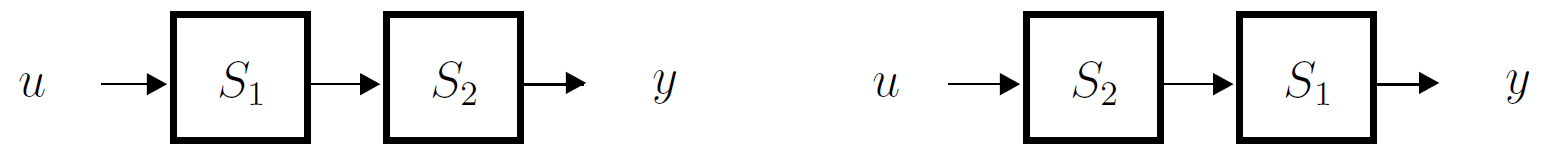
\includegraphics[width=0.85\columnwidth]{images/bloecke_tauschen.png}
\end{center}

Blöcke dürfen \textbf{verschoben werden}, müssen allerdings mit ihrer \textbf{Umkehrfunktion kompensiert werden}, um das Gesamtsystem nicht zu verändern

\begin{center}
	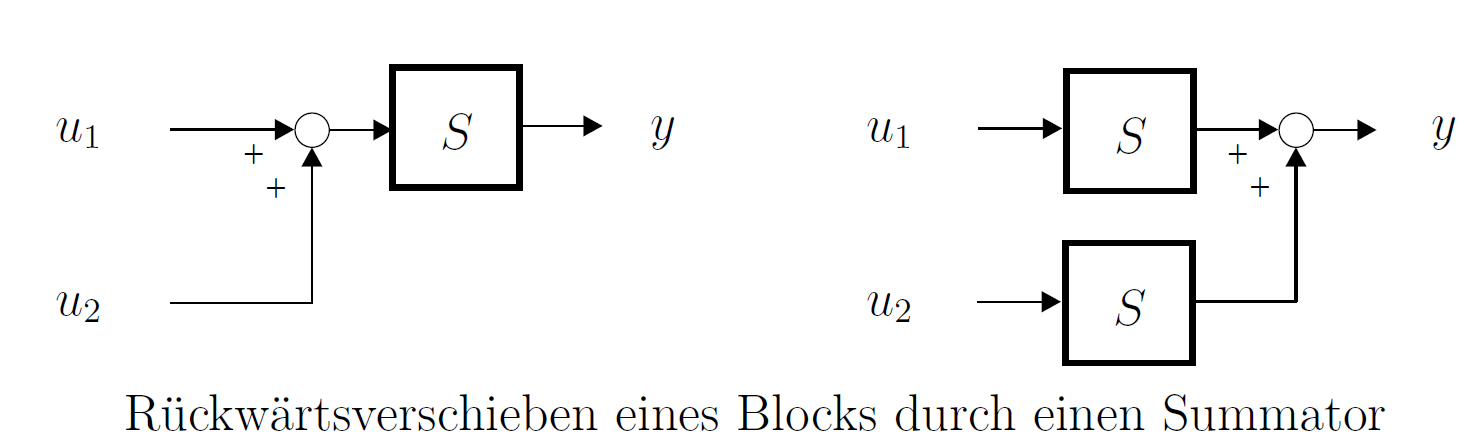
\includegraphics[width=0.73\columnwidth]{images/bloecke_schieben_1.png}
	\vspace{0.2cm}

	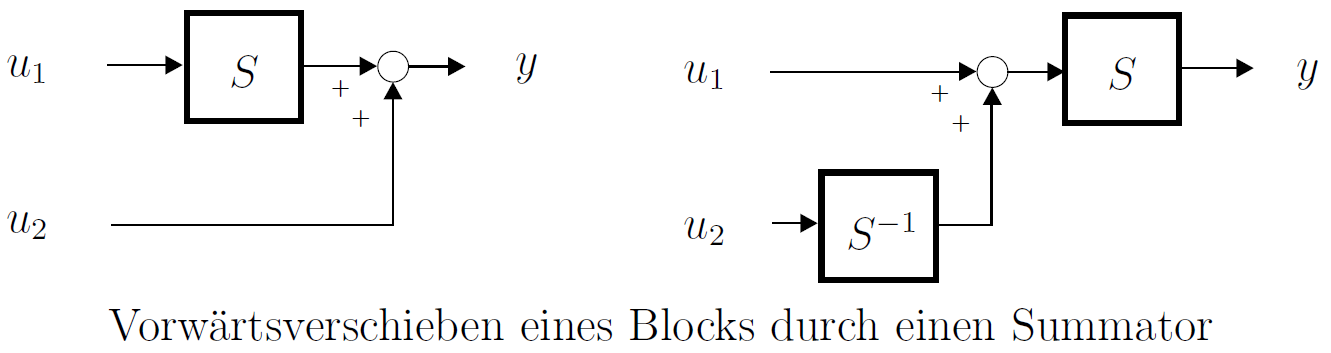
\includegraphics[width=0.73\columnwidth]{images/bloecke_schieben_2.png}
	\vspace{0.2cm}

	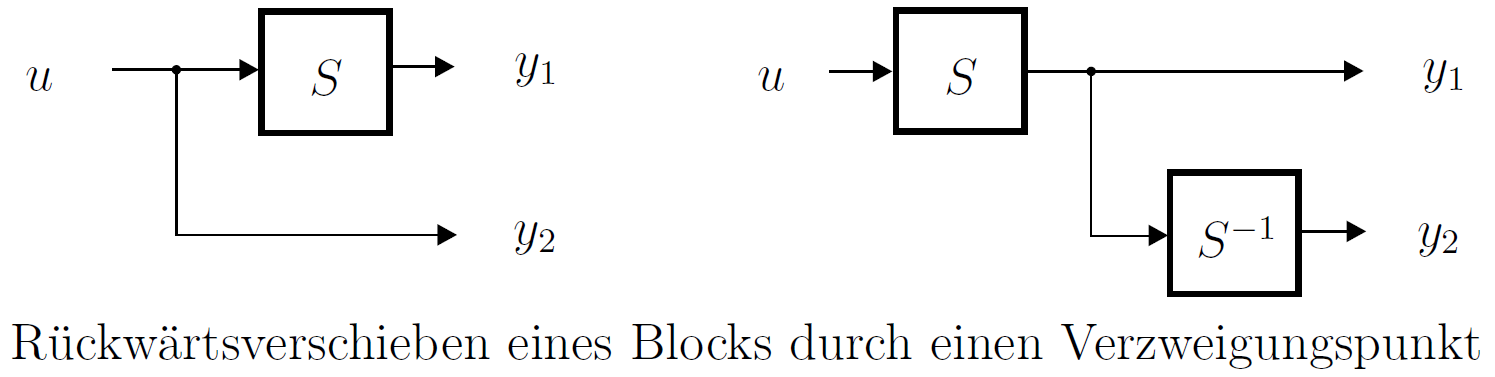
\includegraphics[width=0.73\columnwidth]{images/bloecke_schieben_3.png} 
\end{center}


		\section{Nichtlinearität (NL)}

\subsection{Umgang mit Nichtlinearität und Zeitvarianz}{84}

\begin{minipage}[c]{0.44\columnwidth}
	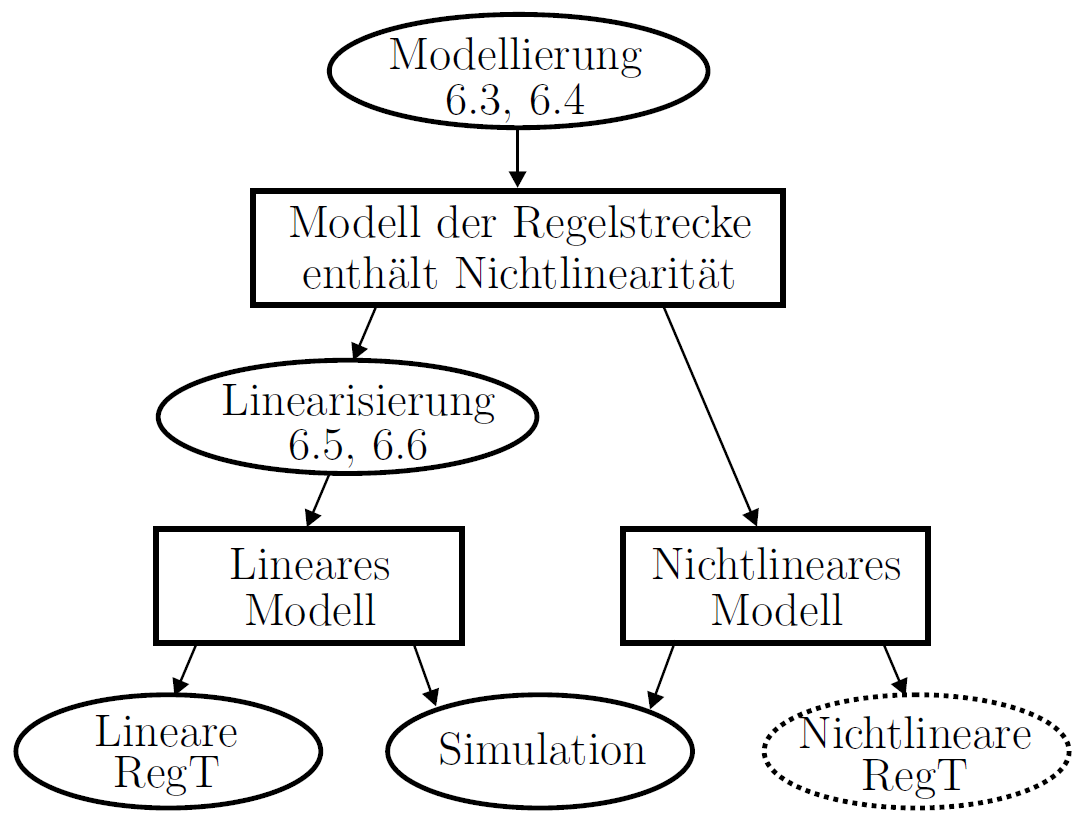
\includegraphics[width=\columnwidth]{images/vorgehen_nichtlineares_streckenmodell.png}
\end{minipage}
\hfill
\begin{minipage}[c]{0.48\columnwidth}
	\raggedright
	Für die Regler-Auslegungmöchten wir \textbf{lineare Systeme}.

	\vspace{0.2cm}

	Reale Systeme sind aber nichtlinear und zeitvariant
	\vspace{0.1cm}

	\begin{outline}
		\1 Sättigungen
		\1 Kennlinien
		\1 Physik
			\2 $F = k \cdot \cbl{i^2}$
			\2 $F = m \cdot g \cdot \cbl{\sin(\varphi)}$ 
	\end{outline}
\end{minipage}


\subsection{Modelle von Nichtlinearitäten (NL)}

Es gibt zwei Modelle, um Nichtlinearität darzustellen:

\vspace{0.2cm}

\begin{minipage}[t]{0.48\columnwidth}
	\textbf{Hammerstein-Modell} 
	\begin{center}
		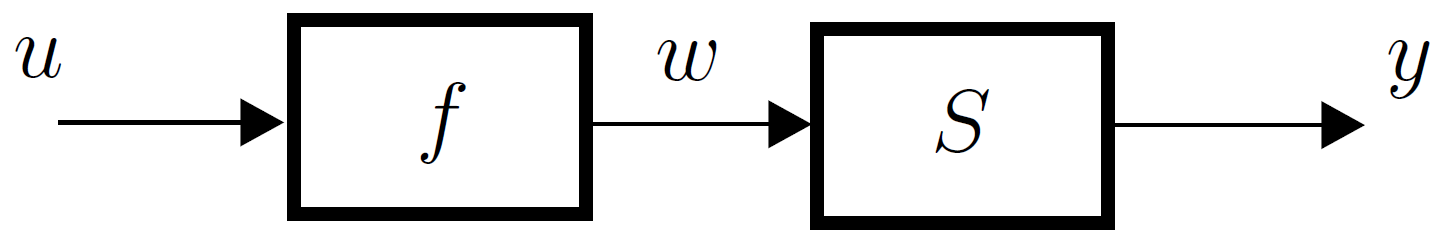
\includegraphics[width=0.9\columnwidth]{images/hammerstein.png}
	\end{center}
\end{minipage} 
\hfill
\begin{minipage}[t]{0.48\columnwidth}
	\textbf{Wiener-Modell} 
	\begin{center}
		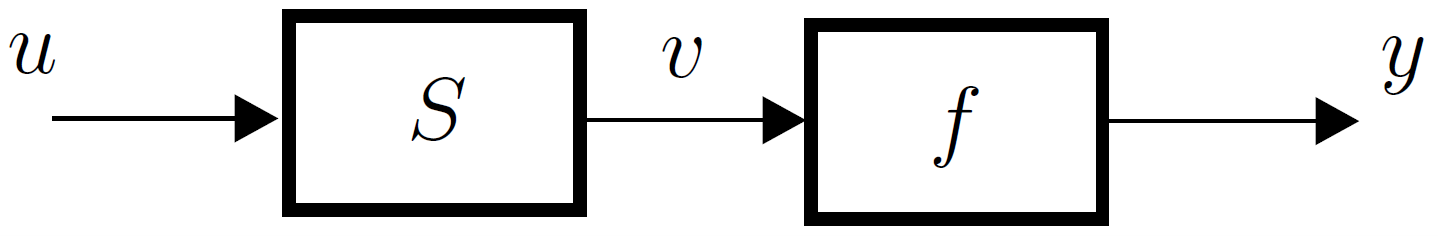
\includegraphics[width=0.9\columnwidth]{images/wiener.png}
	\end{center}
\end{minipage} 

\vspace{0.2cm}

\begin{tabular}{ll}
	$f$ & Nichtlinearität (z.B. Totzeit) 						\\
	$S$ & Stabiles (dynamisches) LZI-System mit Verstärkung 1
\end{tabular}


\subsection[Messung der statischen Kennlinie]{Messung der statischen Kennlinie von $\bm{f}$}{86}

Sowohl für das Hammerstein- als auch für das Wiener-Modell gilt: 
$$ y_{\rm stat} = f(u_{\rm stat}) \qquad \text{(eingeschwungener Zustand)} $$


\subsubsection{Vorgehen statische Messung der einzelnen Punkte}

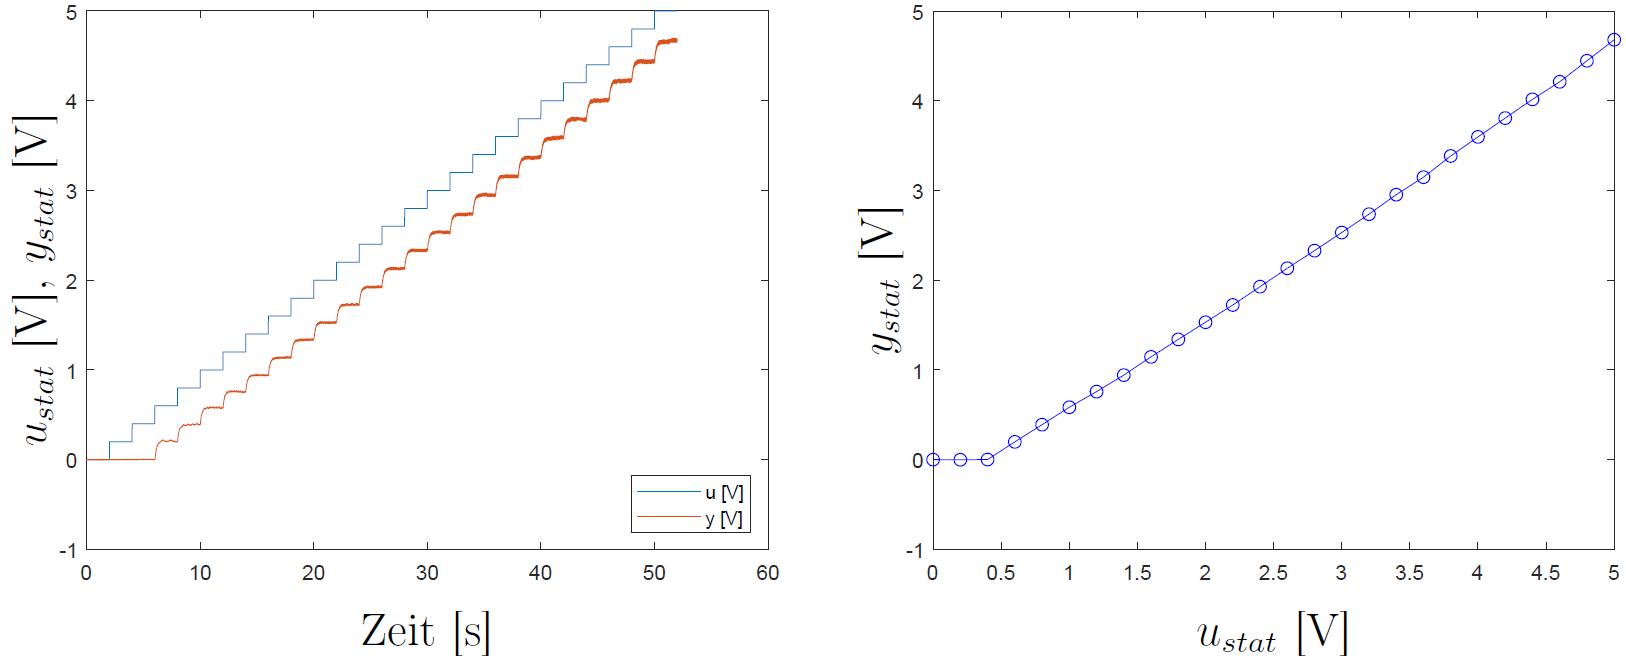
\includegraphics[width=\columnwidth]{images/messung_statische_kennlinie.png}

\begin{itemize}
	\item Eingang $u(t)$ \textbf{schrittweise} ändern (auf neuen Wert $u_{\rm stat}$) Augang $y(t)$ verändert sich stetig und schwingt 
		auf neuen Wert $y_{\rm stat}$ ein (überlagertes Rauschen)
	\item $y_{\rm stat}$ messen (z.B. durch Mittelwertbildung)
	\item Wertepaare $u_{\rm stat}, \, y_{\rm stat}$ ergeben Messpunkte $P_j = (u_j | y_j)$ der Kennlinie
	\item Annahmen über Kennlinie (Totzone, symm. bzgl. Nullpunkt) mit zusätzlichen Messpunkte
		(hier: $u_{\rm stat} > 5 \, V$ bzw. $u_{\rm stat} < 0 \, V$) absichern
\end{itemize}


\subsubsection{Vorgehen dynamische Messung}

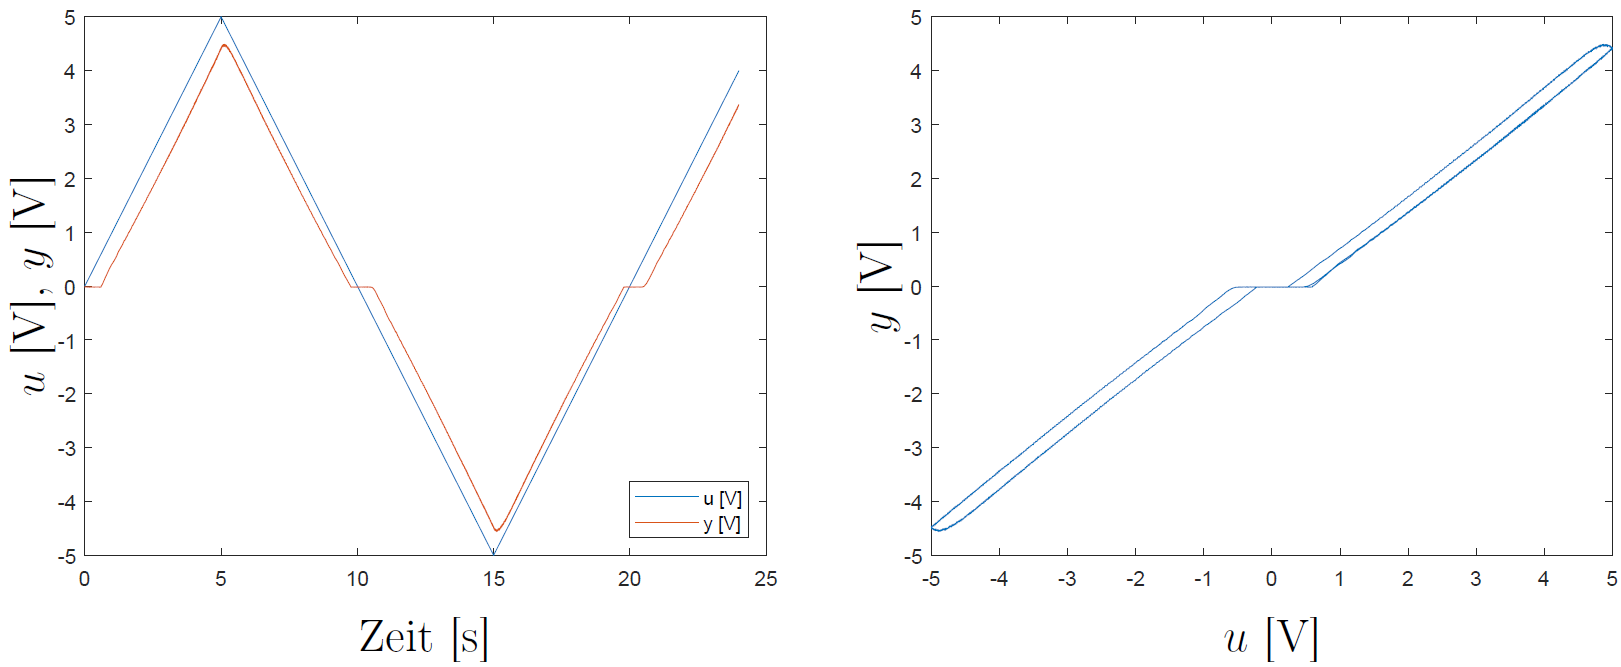
\includegraphics[width=\columnwidth]{images/dynamische_messung_kennlinie.png}

\begin{itemize}
	\item Eingang $u(t)$ \textbf{kontinuierlich} ändern (rampenförmig) \\
		Ausgang $y(t)$ schwingt nicht ein, sondern läuft stationärem Wert stets hinterher \\
		\textrightarrow\ Es entsteht eine \textbf{Pseudohysterese}
	\item Pseudohystere erkennen: Messgeschwindigkeit variieren \\
		\textrightarrow\ $N$ mal langsamere Messung \textrightarrow\ $N$ mal schmalere Hysterese
\end{itemize}


\subsection{Erfassung der NL -- Tabelle}

Die Messung der statischen Kennlinie von $f$ liefert Messpunkte $P_j = (u_j | y_j)$ mit $j = 1 \, ... \, N$ \\
Im einfachsten Fall werden diese Messpunkte als \textbf{Lookup-Table (LUT)} gespeichert.

\vspace{0.2cm}

Diese Form der Datenerfassung kann vor allem bei \textbf{vektoriellen Eingängen} (mehrere Eingangssignale) problematisch werden (Speicherplatz)


\subsection[Erfassung der NL -- Funktion]{Erfassung der NL -- Funktion $\bm{y = f(u)}$}

Eine Kennlinie stellt eine kompaktere Form der Datenerfassung dar. \\
Die Motivation kann auch darin liegen, dass Kennlinien einen \textbf{bekannten physikalischen Effekt} repräsentieren und es nun darum geht,
\textbf{einen oder mehrere Parameter} zu bestimmen.

\vspace{0.2cm}

\textbf{Gesucht wird also eine \textbf{gut passende Funktion} $y = f(u)$}

\vspace{0.1cm}

\begin{itemize}
	\item Idealerweise $y_j = f(u_j) \, \forall j$
	\item Struktur von $f$ beruht auf physikalischem Vorwissen oder möglichst einfache Struktur von $f$
\end{itemize}


\subsubsection{Gleichungssysteme ohne Lösungen}

Hat ein Gleichungssystem keine Lösung (überbestimmt), so führt man einen Fehlerterm $\varepsilon$ in die Gleichung ein:
$$ y_i = f(u_i) = \sum\limits_{i=1}^M \theta_i \cdot f_i(u_j) + \varepsilon_j $$
Nun kann eine Lösung für $\theta$ gesucht werden, bei der dieser Fehler möglichst klein werden (\textbf{\textrightarrow\ Least Squares}) \\
Beispielsweise wird dabei die Zielfunktion $J(\varepsilon) =  \sum\limits_{i=1}^M \varepsilon_i^2$ minimiert.


\subsubsection{Funktion linear in Parametern (l.i.p.)}

Eine Funktion $f$ ist l.i.p. , falls sie die folgenden Form hat.
$$ y = f(u) = \theta_1 \cdot f_1(u) + \theta_2 \cdot f_2(u) + ... = \sum\limits_{i=1}^M \theta_i \cdot f_i(u_j) $$ 
Die Werte $\theta_i$ sind dabei die unbekannten Parameter.


\example{l.i.p. Gleichungssystem mit eindeutiger Lösung}

\vspace{-0.2cm}

$$ \text{Ansatz:} \quad  \cgn{y} = f(u) = \theta_1 \cdot \cbl{u} + \theta_2 \cdot \cor{u^2} \text{ mit 2 Messpunkten } (\cbl{u_j} \, | \, \cgn{y_j}) $$
$$ \begin{vmatrix} \cgn{1.0} = \theta_1 \cdot \cbl{0.8} + \theta_2 \cdot \cor{0.64} \\ \cgn{2.0} = \theta_1 \cdot \cbl{3.0} + \theta_2 \cdot \cor{9.0} \end{vmatrix}
\text{ \textrightarrow\ } \underbrace{ \begin{bmatrix} \cgn{1.0} \\ \cgn{2.0} \end{bmatrix} }_{\substack{y}} = \underbrace{ 
\begin{bmatrix} \cbl{0.8} & \cor{0.64} \\ \cbl{3.0} & \cor{9.0} \end{bmatrix} }_{\substack{\Phi}} \, \underbrace{\begin{bmatrix}  \theta_1 \\ \theta_2 \end{bmatrix} }_{\substack{\theta}}$$
$$ \theta = \Phi^{-1} \cdot y = \underbrace{  \frac{1}{0.8 \cdot 9.0 - 3.0 \cdot 0.64} \begin{bmatrix} 9.0 & -0.64 \\ -3.0 & 0.8 \end{bmatrix} }_{\substack{\Phi^{-1}}}
\, \begin{bmatrix} 1.0 \\ 2.0 \end{bmatrix} = \begin{bmatrix} 1.46 \\ -0.27 \end{bmatrix}$$


\example{l.i.p. überbestimmtes Gleichungssystem}

\vspace{-0.2cm}

$$ \text{Ansatz:} \quad \cgn{y} = f(u) = \theta_1 \cdot \cbl{u} + \theta_2 \cdot \cor{u^2} \text{ mit 3 Messpunkten } (\cbl{u_j} \, | \, \cgn{y_j}) $$
$$ \begin{vmatrix} \cgn{1.0} = \theta_1 \cdot \cbl{0.8} + \theta_2 \cdot \cor{0.64} \\  \cgn{2.5} = \theta_1 \cdot \cbl{2.0} + \theta_2 \cdot \cor{4.0} \\ 
\cgn{2.0} = \theta_1 \cdot \cbl{3.0} + \theta_2 \cdot \cor{9.0} \end{vmatrix} \text{ \textrightarrow\ } 
\underbrace{ \begin{bmatrix} \cgn{1.0} \\ \cgn{2.5} \\ \cgn{2.0} \end{bmatrix} }_{\substack{y}} = 
\underbrace{ \begin{bmatrix}  \cbl{0.8} & \cor{0.64} \\ \cbl{2.0} & \cor{4.0} \\ \cbl{3.0} & \cor{9.0} \end{bmatrix} }_{\substack{\Phi}} \,
\underbrace{\begin{bmatrix}  \theta_1 \\ \theta_2 \end{bmatrix} }_{\substack{\theta}}$$
$$ \boxed{ \theta_{\rm opt} = \underbrace{ (\Phi^T \Phi)^{-1} \Phi^T }_{\substack{P}} \cdot y  \quad \text{(Least Squares)} } $$


\myul{\textbf{Moore-Penrose'sche Pseusodinverse $P$ in Matlab:}}
%DONE: listings
\mylstbox{theta = phi \\ y}
% \textbf{Matlab:} $\boldsymbol{\theta = \Phi \backslash y}$


\subsubsection{Funktion nichtlinear in Parametern (nicht l.i.p.)}

\example{Nicht l.i.p. Gleichungssystem mit mehreren Lösungen}

\vspace{-0.2cm}
$$ \text{Ansatz:} \quad \cgn{y} = f(u) = \theta_1 \cdot \sin( \theta_2 \cdot \cbl{u}) \text{ mit 2 Messpunkten } (\cbl{u_j} \, | \, \cgn{y_j}) $$ 
$$ \begin{vmatrix} \cgn{1.0} = \theta_1 \cdot \sin(\cbl{0.8} \cdot \theta_2 ) \\  \cgn{2.0} = \theta_1 \cdot \sin(\cbl{3.0}  \cdot \theta_2 ) \end{vmatrix} 
\text{ \textrightarrow\ } \frac{ (\Romannum{1}) }{(\Romannum{2}) } \text{ \textrightarrow\ }
0.5 = \frac{\sin(\cbl{0.8} \cdot \theta_2)}{\sin(\cbl{3.0}  \cdot \theta_2 )} $$

Sinus-Term plotten und mehrere Schnittpunkte (Lösungen) finden


\example{Nicht l.i.p. Gleichungssystem}

\vspace{-0.2cm}
$$ \text{Ansatz:} \quad \cgn{y} = f(u) = \theta_1 \cdot \sin( \theta_2 \cdot \cbl{u}) \text{ mit 3 Messpunkten } (\cbl{u_j} \, | \, \cgn{y_j}) $$
$$ \begin{vmatrix} \cgn{1.0} = \theta_1 \cdot \sin(\cbl{0.8} \cdot \theta_2 ) + \varepsilon_1 \\ \cgn{2.5} 
= \theta_1 \cdot \sin(\cbl{2.0}  \cdot \theta_2 )  + \varepsilon_2  \\ \cgn{2.0} 
= \theta_1 \cdot \sin(\cbl{3.0}  \cdot \theta_3 )  + \varepsilon_2\end{vmatrix}  \text{ \textrightarrow\ Fehler minimieren} $$

Es entstehen differentielle Ableitungen mit vielen Sinus-Termen, welche Null gesetzt werden müssen \textrightarrow\ mühsam!

\vspace{0.2cm}
\textbf{Man verwendet besser ein lineares Modell, dann gibt es auch nur eine Lösung!}


\subsection{Linearisierung durch Veränderung der Strecke}

\subsubsection{Inversion der Kennlinie}

Um die Nichtlinearität $f$ in der Strecke zu kompensieren wird am Ausgang des Reglers die 
\textbf{Umkehrfunktion der Nichtlinearität} $f^{-1}$ eingefügt.\\
Somit wird $w = \tilde{u}$ und der Regler hat nur das $\text{PT}_1$-Glied als Regelstrecke 

\begin{center}
	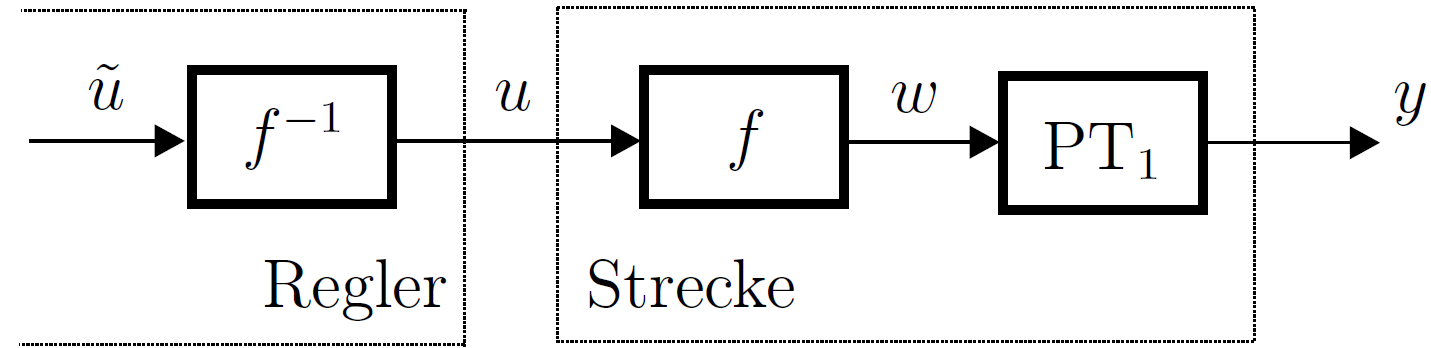
\includegraphics[width=0.7\columnwidth]{images/linearisierung_inversion_kennlinie.png}
\end{center}


Egal wo die Nichtlinearität ist, es muss am 'passenden Ort' im Blockdiagramm die \textbf{Umkehrfunktion der Nichtlinearität} eingefügt werden. \\
\textrightarrow\ ggf. Verschiebungsregeln aus Kapitel ~\ref{Serieschaltung von LZI-Systemen} anwenden 

\vspace{0.2cm}

\textbf{Bemerkungen} 
\vspace{0.1cm}

\begin{itemize}
	\item $f$ kann nicht in allen Fällen invertiert werden \\
		 \textrightarrow\ Sättigungen am Streckeneingang besitzt kein $f^{-1}$ 
	\item Es muss nicht zwischen Wiener- und Hammersein-Struktur unterschieden werden\\
		\textrightarrow\ Gleiches Vorgehen 
\end{itemize}


\subsubsection{Gegenkopplung unterlagerte Regler}

Ein Regler hält den Fehler $e$ bei $0$. Schafft er das, dann ist $y(t) \approx r(t)$ und somit das Gesamtverhalten 'einigermassen' linear.

\begin{center}
	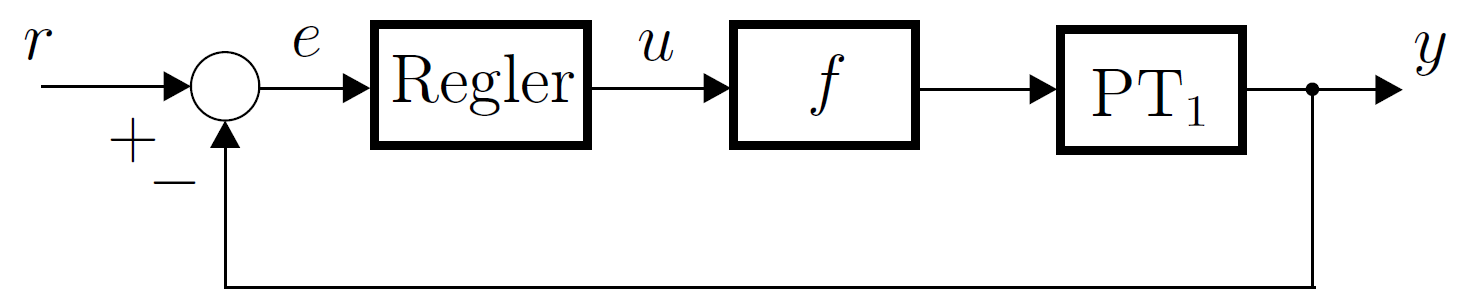
\includegraphics[width=0.7\columnwidth]{images/unterlagerte_regelung.png}
\end{center}


\begin{itemize}
	\item  Überlagerter Regler 'sieht' ein einfaches P-Glied mit $K = 1$ \\
		\textrightarrow\ \textbf{Unterlagerter (linearisierender) Regler} muss \textbf{schneller} sein als überlagerter Regler
		\item Kaskadenreglung 
\end{itemize}

\vspace{0.2cm}
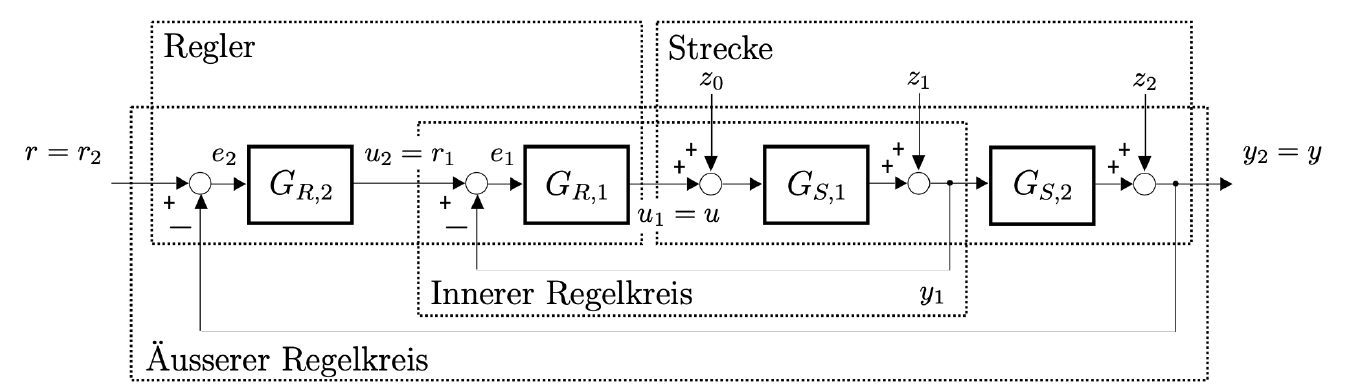
\includegraphics[width=\columnwidth]{images/kaskadenregelung}


\subsection{Linearisierung durch Vereinfachung}{94}

Idee: In einem Arbeitspunkt verhält sich das System 'genügend' linear\\
\textrightarrow\ konstanter Wert \textbf{(steady state)} 


\subsubsection{Steady State}

Ist ein System im 'Steady State', so gilt: 
\vspace{0.1cm}

\begin{minipage}[t]{0.48\columnwidth}
	\begin{itemize}
		\item Fehler $e(t) = 0 $
	\end{itemize}
\end{minipage}
\hfill
\begin{minipage}[t]{0.48\columnwidth}
	\begin{itemize}
		\item Ableitungen $= 0$ 
	\end{itemize}
\end{minipage}


\subsubsection{Vorgehen Linearisierung im Arbeitspunkt}

\begin{minipage}{0.48\columnwidth}
	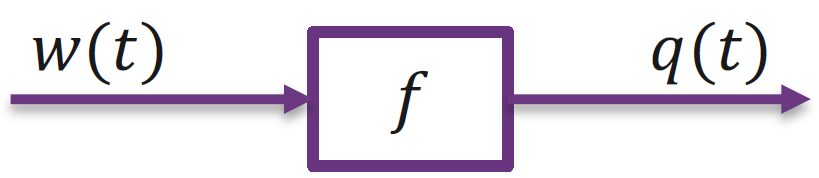
\includegraphics[width=0.7\columnwidth]{images/linearisierung_vereinfachung_1.png} 
\end{minipage}
\hfill
\begin{minipage}{0.48\columnwidth}
	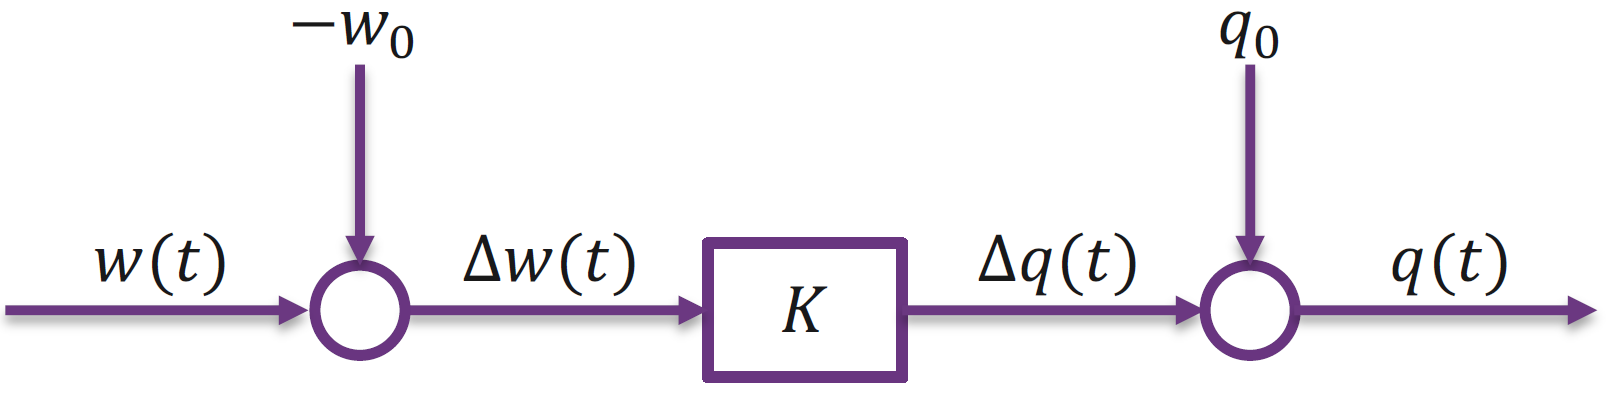
\includegraphics[width=\columnwidth]{images/linearisierung_vereinfachung_2.png} 
\end{minipage}

\vspace{0.2cm}

\begin{enumerate}
	\item Alle Signale durch $x(t) = x_0 + \Delta x(t)$ ersetzen \\
		(Nominalwerte $x_0 = \text{const}$ und kleine Abweichung $\Delta x(t)$)
	\item Nominalwert $x_0$ festlegen / bestimmen \\
		\textrightarrow\ Typischerweise der Sollwert $y_0$ für Regelgrösse $y$
	\item \cgn{Signale im Blockdiagramm durch $\Delta x(t)$ ersetzen}
	\item \cbl{Anpassung Eingang: $w(t) = \Delta w(t) - w_0$ (Subtraktion)} \\
		\crd{Anpassung Ausgang: $q(t) = q_0 + \Delta q$ (Addition)}
	\item Lineare Blöcke übernehmen
	\item \cor{Nichtlineare Blöcke durch Näherungen (z.B. Gain) ersetzen \textrightarrow\ \textbf{Steady-State} beachten} 
		\begin{itemize}
			\setlength\itemsep{0.75em}
			\item $q(t) = f(w(t)) \;$ \textrightarrow\ $\Delta q(t) = K \cdot \Delta w(t)$
			\item $K = \frac{\diff q}{\diff w} \Big|_{w=w_0}$ (Steigung im Arbeitspunkt) 
			\item $\bm{q(t) \approx q_0 + K \cdot \Delta w(t) = q_0 + K \cdot (w(t) - w_0)$} \quad \textrightarrow\ $\bm{q_0 = q(t_0)}$
		\end{itemize}
\end{enumerate}

   
\example{Linearisierung Auto}   
\begin{center}
	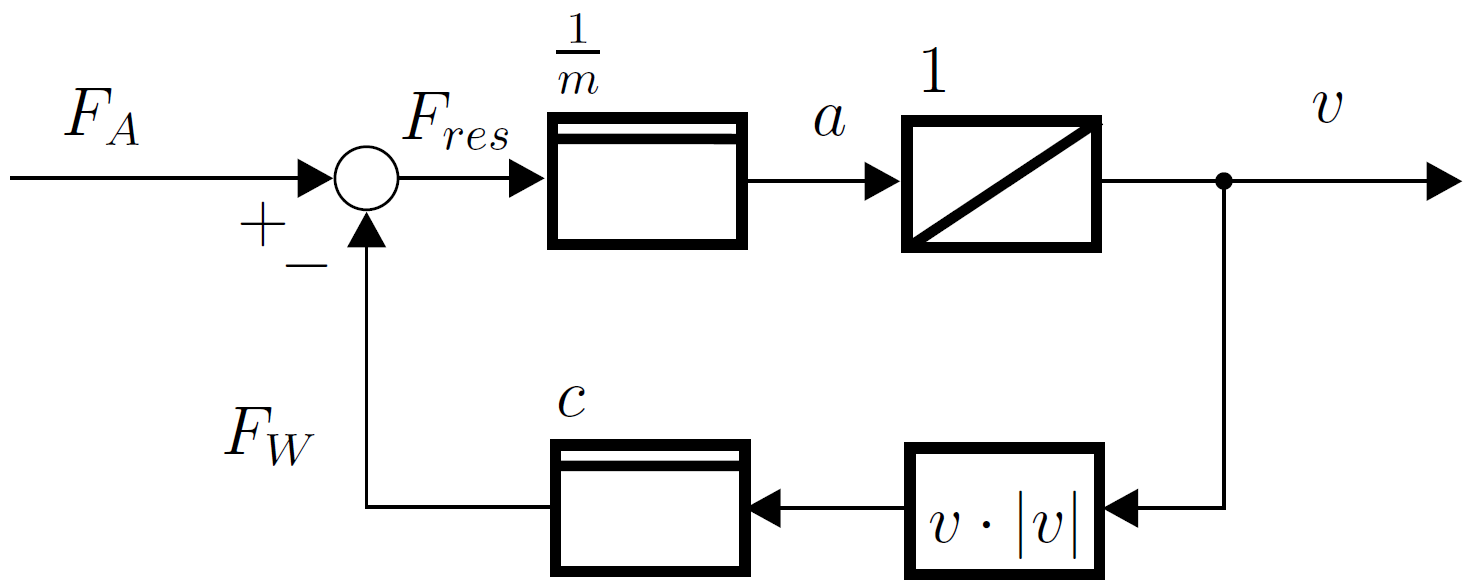
\includegraphics[width=0.6\columnwidth]{images/beispiel_linearisierung_1.png}
	\vspace{0.2cm}
	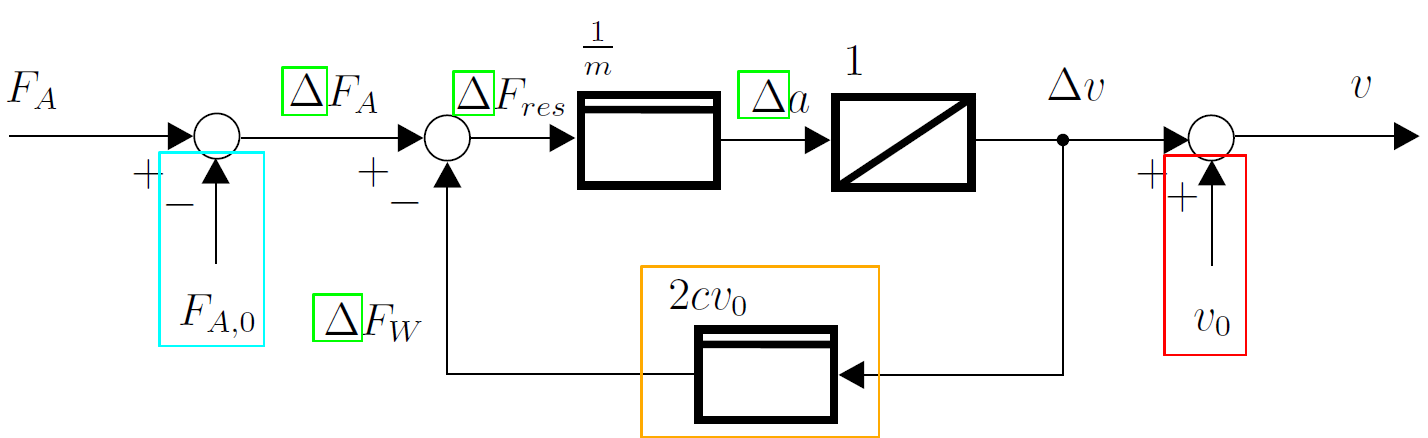
\includegraphics[width=0.8\columnwidth]{images/beispiel_linearisierung_2.png}
\end{center}

\vspace{-0.2cm}

\renewcommand{\arraystretch}{1.8}
\begin{tabular}{l}
	Nominalgeschwindigkeit: $v_0 > 0 = \const$ \\
	$v_0 = \const$ \quad \textrightarrow\ $a_0 = 0$ \quad \textrightarrow\ $F_{ \rm res, 0} = 0 $ \\
	$ F_{A,0} = F_{W,0}$ \quad \textrightarrow\ $F_{W,0} = c \cdot v_0^2$ \quad \textrightarrow\ $ F_{A,0} = c \cdot v_0^2$ 
\end{tabular}
\renewcommand{\arraystretch}{1}

\vspace{0.2cm}

\myul{\textbf{Rechenweg Linearisierung}}

\vspace{0.2cm}

\begin{minipage}[c]{0.34\columnwidth}
	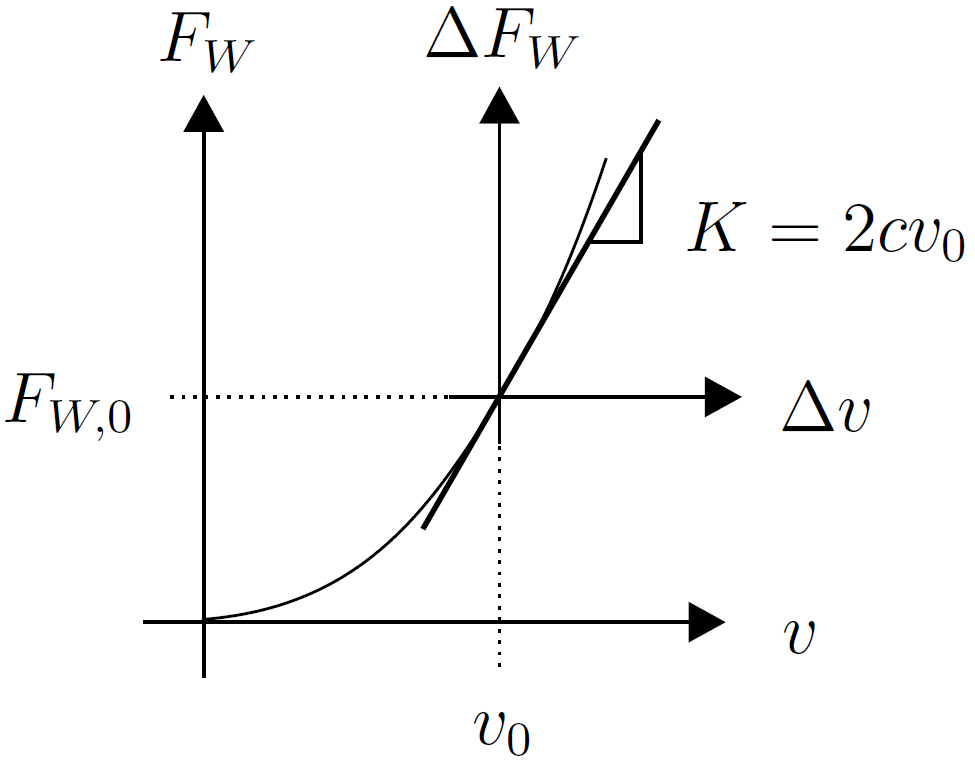
\includegraphics[width=\columnwidth]{images/beispiel_linearisierung_3.png} 
\end{minipage}
\hfill
\begin{minipage}[c]{0.58\columnwidth}
		$$ F_W = c \cdot v^2 $$
		$$ \frac{\diff F_W}{\diff v} \big| _{v = v_0} = c \cdot 2 \cdot v \big| _{v = v_0} = \underbrace{2 \, c \, v_0}_{K} $$
		$$ \Delta F_W \approx K \cdot \Delta v $$
\end{minipage}


		\section{Diverses}

\subsection{'Control'-Fragen}

\subsubsection{Wieso Feedback?}

Closed-Loop Control (Regelung) statt Open-Loop Control (Steuerung)


\subsubsection{Vorteile / Nachteile einer Steuerung}

\begin{itemize}
	\item[-] Störung $Z$ muss bekannt sein
	\item[-] Anfangswert $x_0$ muss bekannt sein
	\item[-] Struktur und Parameter des Modells müssen bekannt sein
	\item[-] (Steuer-) Strecke muss stabil sein
	\item[+]    Braucht keinen Sensor 
\end{itemize}


\subsubsection{Wozu ein Modell erstellen?}

 \begin{itemize}
	\item Steuerung: Braucht sowieso ein Modell
	\item Regelung: Modellierung von Sensor \textbf{muss} gut sein
	\item Falsches Modell kann Regler destabilisieren (Schwingung)
 \end{itemize}


\subsubsection{Vorteile linearer Modelle?}

\begin{itemize}
	\item Für lineare Modelle (lineare DGL) gibt es Standardverfahren zur Lösung 
	\item Die Systeme sind (grundsätzlich immer) lösbar
\end{itemize}



\section{Physik Formeln}

Um die DGL eines Systems aufzustellen könnten die folgenden Formeln aus der Physik hilfreich sein.


\subsection{Statik}

\subsubsection{Schiefe Ebene}

\begin{center}
    \begin{tikzpicture}
		%Raster im Hintergrund
		%\draw[step=1, gray, very thin] (0,0) grid (7,6);	

		%Grunddreieck	
		\draw [fill=gray!20] (0,0) -- (7,0) -- (7,4.04145) -- (0,0);
		
		%Winkel
		\filldraw[fill=blue!10, draw=blue!50!black, thick] (0,0) -- (1.5,0) arc(0:30:1.5) node [midway, xshift=-10pt, yshift=-3, blue!50!black] {$\alpha$} {};
				
		\draw [very thick] (0,0) -- (7,0) -- (7,4.04145) -- (0,0);
				
		%Bezugssystem
		\begin{scope}[xshift=1cm, yshift=3cm, rotate=30, scale=1]
	    	%Länge x Achse
			\draw [-latex, thick] (0,0) -- ++(1,0) node[below, rotate=30] {$x$};
		
			%Länge y Achse
			\draw [-latex, thick] (0,0) -- ++(0,1) node[left, rotate=30] {$y$};
  		\end{scope}
  		
  		%Alles was gedreht wurde (Masse m, Kräftevektoren, ...)
		\begin{scope}[xshift=3.464cm, yshift=2cm, rotate=30, scale=1.1]

			\coordinate (A) at (0.75,0.5);
			\coordinate (B) at (0.75,-1.5);
			
			%Rechteck
			\draw [fill=orange!20!white] (0,0) rectangle (1.5,1);
			\draw [orange, very thick] (0,0) rectangle (1.5,1) node [midway, right, xshift=3pt, yshift=3pt] {$m$} {} ;
			%Vektor FR
			%\draw [-latex, very thick, purple] (0,0) -- ++ (-1.5,0) node [midway, above, yshift=3pt] {$\vec{F}_R$} {};
			
			%Vektoren Kraft-Seil
			\begin{scope}[xshift=1.5cm, yshift=1cm, rotate=0, scale=1]
    			\begin{scope}[xshift=0cm, yshift=0cm, rotate=0, scale=1]
    				%\filldraw[fill=green!10, draw=green!50!black, thick] (0,0) -- (1,0) arc(0:33.6900:1) 
    					%node [midway, left, xshift=0pt, yshift=-7, green!50!black] {$\beta$} {};
    			\end{scope}
    			\coordinate (C) at (1.5,0);
				\coordinate (D) at (1.5,1);
				%Rechter Winkel
				%\draw [thick](1.2,0) -- (1.2,0.3) -- (1.5,0.3);
    			\draw [-latex, very thick, purple] (0,-1) -- ++ (C) node [midway, below] {$\vec{F}_{R}$} {};
				%\draw [-latex, very thick, green!50!black] (C) -- ++ (0,1) node [midway, right] {$\vec{F}_{Sy}$} {};
				%\draw [-latex, very thick, red] (0,0) -- ++ (D) node [midway, left] {$\vec{F}_S$} {};
				%Rechter Winkel
    			  
    		\end{scope}	
			
			%Vektoren FN, FG, FH
    		
    		\begin{scope}[xshift=0cm, yshift=0, rotate=0, scale=1]
    			\coordinate (A) at (0.75,0.5);
				\coordinate (B) at (0.75,-1.5);
    			\begin{scope}[xshift=0.75cm, yshift=0.5cm, rotate=-120, scale=1]
    				\filldraw[fill=blue!10, draw=blue!50!black, thick] (0,0) -- (1,0) arc(0:30:1) 
    					node [midway, above, xshift=-1.5pt, yshift=0, blue!50!black] {$\alpha$} {};
    			\end{scope}
    			%Rechter Winkel
    			\draw [thick](0.45,-1.5) -- (0.45,-1.2) -- (0.75,-1.2);  
    			\draw [-latex, very thick, dashed, green!50!black] (B) -- (A) node [midway, right] {$\vec{F}_N$} {};
				\draw [-latex, very thick, green!50!black] (A) -- ++(0,2) node [midway, right] {$\vec{F}_N$} {};
    			\draw [-latex, very thick, purple] (B) -- ++(-1.1547,0) node [midway, below] {$\vec{F}_H$} {};
    			\draw [-latex, very thick, red] (A) -- ++(-1.1547,-2) node [midway, left] {$\vec{F}_G$} {};
    			%Rechter Winkel
    			\draw [thick](0.45,-1.5) -- (0.45,-1.2) -- (0.75,-1.2);  
    		\end{scope}		    		
  		\end{scope}
	\end{tikzpicture}
\end{center}

\subsubsection*{Formeln und Zusammenhänge zur schiefen Ebene}

\begin{tabular}{llll}
	$F = m \cdot a$	& $F_G = m \cdot g$ &	$F_N = m \cdot g \cdot \cos(\alpha)$ &	$F_H = m \cdot g \cdot \sin(\alpha)$
\end{tabular}
	
	
\subsubsection{Kräftegleichgewicht -- Beispiel}

\begin{minipage}[c]{0.35\columnwidth}
	\begin{align*}
		F_{\rm res} &= F_G + F_R \\
		m \cdot a	&= m \cdot g + F_N \cdot \mu
	\end{align*}
\end{minipage}
\hfill
\begin{minipage}[c]{0.6\columnwidth}
	\textbf{ \textrightarrow\ Reibung ist proportional zur Geschwindigkeit!}
\end{minipage}


\subsection{Kinematik}

\renewcommand{\arraystretch}{1.1}
\begin{tabular}{ll}
	Ort 			& $x$ 						\\
	Geschwindigkeit & $v = \dot{x}$ 			\\
	Beschleunigung 	& $a = \dot{v} = \ddot{x}$
\end{tabular}
\renewcommand{\arraystretch}{1}


\subsubsection{Gleichförmige Bewegung $\bm{a(t) = 0}$}

\renewcommand{\arraystretch}{1.3}
\begin{tabular}{l}
	$a(t) = \ddot{x} = 0$ 			\\
	$v(t) = v_0 = \dot{x} = \const$ \\
	$x(t) = v_0 \cdot t + x_0$
\end{tabular}
\renewcommand{\arraystretch}{1}
		
		
\subsubsection{Gleichmässig beschleunigte Bewegung $\bm{a(t) = \const}$}

\renewcommand{\arraystretch}{1.3}
\begin{tabular}{l}
	$a(t) = a_0 = \ddot{x} = \const$ 							\\
	$v(t) =  \dot{x} = a_0 \cdot t + v_0$ 						\\
	$x(t) = \frac{1}{2} \, a_0 \cdot t^2 + v_0 \cdot t + x_0$
\end{tabular}
\renewcommand{\arraystretch}{1}
	

\subsection{Dynamik}

\subsubsection{Translation vs. Rotation}
\renewcommand{\arraystretch}{1.2}
\begin{tabular}{| c | c |}
	\hline
	\textbf{Translation} 	& \textbf{Rotation}	\\
	\hline
	$a$ 					& $\alpha$ 			\\
	\hline
	$v$ 					& $\omega$ 			\\
	\hline
	$x$ 					& $\theta$ 			\\
	\hline
	$F$ 					& $M$ 				\\
	\hline
	$m$ 					& $J$ 				\\
	\hline
\end{tabular}
\renewcommand{\arraystretch}{1}


\subsubsection{Leistung}

\vspace{-0.2cm}
$$ \boxed{ P = \dot{W} = F \cdot v } $$


\subsubsection{Arbeit / Energie}

\vspace{-0.2cm}
$$ \boxed{ W = F \cdot s } $$

\subsubsection{Energieerhaltung}

\vspace{-0.2cm}
$$ \boxed{ W = \underbrace{m \cdot g \cdot h}_{\substack{\text{pot. Energie}}} =  m \cdot g \cdot \underbrace{ \frac{1}{2} \, g \cdot t^2}_{\substack{\text{h(t)}}}  = \underbrace{ \frac{1}{2} m \cdot v^2 }_{\substack{\text{kin. Energie}}} } $$ 
\vspace{0.2cm}


\myul{\textbf{Energiesatz der Mechanik}}
$$ \boxed{ E_{\rm pot} + E_{\rm kin} = E_{\rm tot} = \const} \qquad \text{(gilt zu jedem Zeitpunkt)} $$


\subsection{Hydrodynamik}

\subsubsection{Induzierter Widerstand $F_W$}

Induzierter Widerstand = Luftwiderstand 

$$ \boxed{ F_W = c^*_W \cdot \frac{1}{2} \cdot \rho \cdot v^2 \cdot A_{\|} } $$

\renewcommand{\arraystretch}{1.3}
\begin{tabular}{c l c}
		$F_W$ 		& Induzierter Widerstand 								& $[F_W] = \newton$ 						\\
		$c^*_W$ 	& Widerstands-Koeffizient 								& $[c*_W] = 1$ 								\\
		$\rho$ 		& Luft-Dichte		 									& $[\rho] = \frac{\kilo \gram}{\meter^3}$ 	\\
		$v$ 		& Strömungsgeschwindigkeit 								& $[v] = \frac{\meter}{\second}$ 			\\
		$A_{\|}$ 	& Projizierte Fläche \textbf{parallel} zur Strömung 	& $[A_{\|}] = \meter^2$
\end{tabular}
\renewcommand{\arraystretch}{1}


\subsection{Thermodynamik}

\subsubsection{Wärme}

\vspace{-0.2cm}
$$ \boxed{ \Delta P = \Delta \dot{Q}} $$


\subsubsection{Wärmekapazität}

\vspace{-0.2cm}
$$ \boxed{ \Delta Q = c \cdot m \cdot \Delta T = n \cdot C_m \cdot \Delta T = C \cdot \Delta T }$$


\subsubsection{Absolute Wärmekapazität $C$}

Energiespeicher-Vermögen eines \textbf{Gegenstands}
$$ \boxed{ \Delta Q = C \cdot \Delta T } $$


\subsubsection{Spezifische Wärmekapazität $c$}

Energiespeicher-Vermögen einer \textbf{Substanz}
$$ \boxed{ \Delta Q = c \cdot m \cdot \Delta T  } \qquad \qquad c_{\rm Wasser} = 4187 \, \frac{\joule}{\kilo \gram \cdot \kelvin} $$


\subsubsection{Molare Wärmekapazität $C_m$}

Energiespeicher-Vermögen einer \textbf{Anzahl Moleküle}
$$ \boxed{ C_m = \frac{c}{n} = M \cdot c } $$

\renewcommand{\arraystretch}{1.3}
\begin{tabular}{c l c}
	$\Delta Q$ 	& Zu-/Abgeführte Wärme 			& $[\Delta Q] = \joule$ 							\\
	$c$ 		& Spezifische Wärmekapazität 	& $[c] = \frac{\joule}{\kilo \gram \cdot \kelvin}$ 	\\
	$C$ 		& Absolute Wärmekapazität 		& $[C] = \frac{\joule}{\kelvin}$ 					\\
	$C_m$ 		& Molare Wärmekapazität 		& $[C_m] = \frac{\joule}{\mole \cdot \kelvin}$ 		\\
	$m$ 		& Masse 						& $[m] = \kilo \gram$ 								\\
	$\Delta T$ 	& Temperaturänderung 			& $[\Delta T] = \kelvin$ 							\\
	$n$ 		& Mol-Zahl 						& $[n] = \mole$ 									\\
	$M$ 		& Mol-Masse 					& $[M] = \frac{\kilo \gram}{\mole}$
\end{tabular}
\renewcommand{\arraystretch}{1}


    \end{layout}
\end{document}

